%% Chapter 12 — Scaling and Cost Optimization
\setcounter{chapter}{11}
\chapter{Scaling and Cost Optimization}
\chaptersubtitle{Autoscaling, cold starts, shared silicon, and the FinOps portfolio — the fleet learns to breathe, and the bill finally lands}

\begin{calloutbox}{tbbblue}{tbbbluefill}
{\normalsize\bfseries\color{tbbblue}Learning objectives}\par\vspace{3pt}
\begin{tbbitemize}
  \item Read a fleet's day as a \textbf{load-factor problem} (needed ÷ paid replica-hours), price the idle gap, and explain why serving's economics were solved conceptually by electric utilities a century ago.
  \item Wire an autoscaler to the \textbf{right metric} — the queue users feel, not the CPU\% nobody uses — and operate the HPA/KEDA control loop: the desire formula, stabilization windows, scheduled scaling, scale-to-zero.
  \item Itemize the \textbf{GPU cold start} (schedule, image, weights, engine, warm-up; ×3 if a node must be born), place Firecracker's 125 ms in that bill correctly, and climb the mitigation ladder rung by rung.
  \item Choose among \textbf{time-slicing, MPS, and MIG} by isolation need — and compute when a slice of a big card beats a whole small one.
  \item Position \textbf{KServe}: the platform layer that operates Chapters 5–11 from one CRD — and when a raw Deployment + KEDA is the smarter choice.
  \item Assemble the \textbf{pricing portfolio} (committed floor, on-demand shoulder, spot burst, off-peak fill), walk the project's bill from \$2,381 to under the \$900 ceiling with receipts, and close Chapter 1's build-vs-buy break-even with measured \$/M-token numbers — the midpoint package.
\end{tbbitemize}
\end{calloutbox}

\vspace{2.5pt}

\begin{calloutbox}{tbbteal}{tbbtealfill}
{\normalsize\bfseries\color{tbbteal}Key terms}\par\vspace{3pt}
load factor · diurnal curve · HPA / KEDA · ScaledObject · desired-replica formula · stabilization window · scheduled scaling · scale-to-zero · GPU cold start · pre-warm pool · cluster autoscaler · time-slicing · MPS · MIG · noisy neighbor · KServe / InferenceService · committed use · on-demand · spot/preemptible · drain drill · unit economics (\$/M tokens) · showback
\end{calloutbox}

\vspace{2.5pt}

\begin{calloutbox}{tbblightgray}{tbbboxfill}
{\normalsize\bfseries\color{tbbink}Chapter outline}\par\vspace{3pt}
\textbf{12.1} The bill that never sleeps — and the man who fixed it in 1902    \textbf{12.2} Autoscaling: the right metric and the stopwatch    \textbf{12.3} Cold starts and scale-to-zero    \textbf{12.4} Sharing the silicon: time-slicing, MPS, MIG    \textbf{12.5} KServe and the FinOps portfolio    \textbf{12.6} Lab: the project midpoint — followed by a summary, exercises, and further reading.
\end{calloutbox}

\section{The Bill That Never Sleeps — and the Man Who Fixed It in 1902}

Every technical chapter since Week 7 has made one replica better: honest (9), cheap per token (10), streaming and fully booked (11). Nobody has yet asked the fleet the rude question Chapter 1's Exhibit B asked a single ghost GPU: \textbf{who exactly is using you at 3 a.m.?} The project's four L4 replicas run around the clock because that is what \code{replicas: 4} means — Chapter 5's controllers keep the promise with perfect, expensive diligence, through lunch rushes and through the dead of night. This chapter begins by measuring what that diligence costs, and the measurement is Exhibit 12-A:

\begin{terminalbox}
\begin{Verbatim}[breaklines=true,breakanywhere=true,fontsize=\small,formatcom=\color{tbbtermfg},codes=\tbbcodeactive]
$ python fleet_ledger.py --day yesterday       # measured, not modeled
 hour    streams   replicas needed   running   note
 03:00       8          2*              4      # *floor: rollout safety
 09:00      71          3               4      # morning climb
 13:00     104          4               4      # the only honest hour
 17:00      55          3               4
 22:00      19          2               4

 needed today:  4x4h + 3x5h + 2x15h = 61 replica-hours
 paid today:    4x24h               = 96 replica-hours
 load factor:   61/96 = 63.5%
 monthly:  paid $2,381  =  needed $1,513  +  IDLE $868
# the fleet is sized for 13:00 and billed for 03:00.
# Exhibit 1-B's ghost GPU, diurnal edition: $868/mo of night shift.
\end{Verbatim}
\end{terminalbox}
\figcaption{Exhibit 12-A  One measured day. The fleet is provisioned for its best hour and billed for all of them; thirty-five replica-hours a day serve nobody. Load factor — needed over paid — is the one number this chapter exists to raise.}

Note what kind of problem this is: \textbf{nothing is misconfigured}. Every replica is optimized, gated, honest. The waste is structural — demand has a \textit{shape} in time (Chapter 1 called serving traffic "decided by users," and users sleep), while the fleet is a horizontal line. Chapter 7's think-box had you estimate this gap on paper ("what does Week 12 owe you?"); Exhibit 12-A is that estimate, measured. And the fix cannot be another per-replica lever: Chapter 10 made requests cheaper, Chapter 11 made seats fuller, but a \textit{provisioned-and-idle} replica burns \$0.80 an hour at any efficiency. The remaining lever moves the \textbf{count}.

\begin{tbbfigure}
  \adjustbox{max width=0.94\linewidth,max totalheight=0.46\textheight}{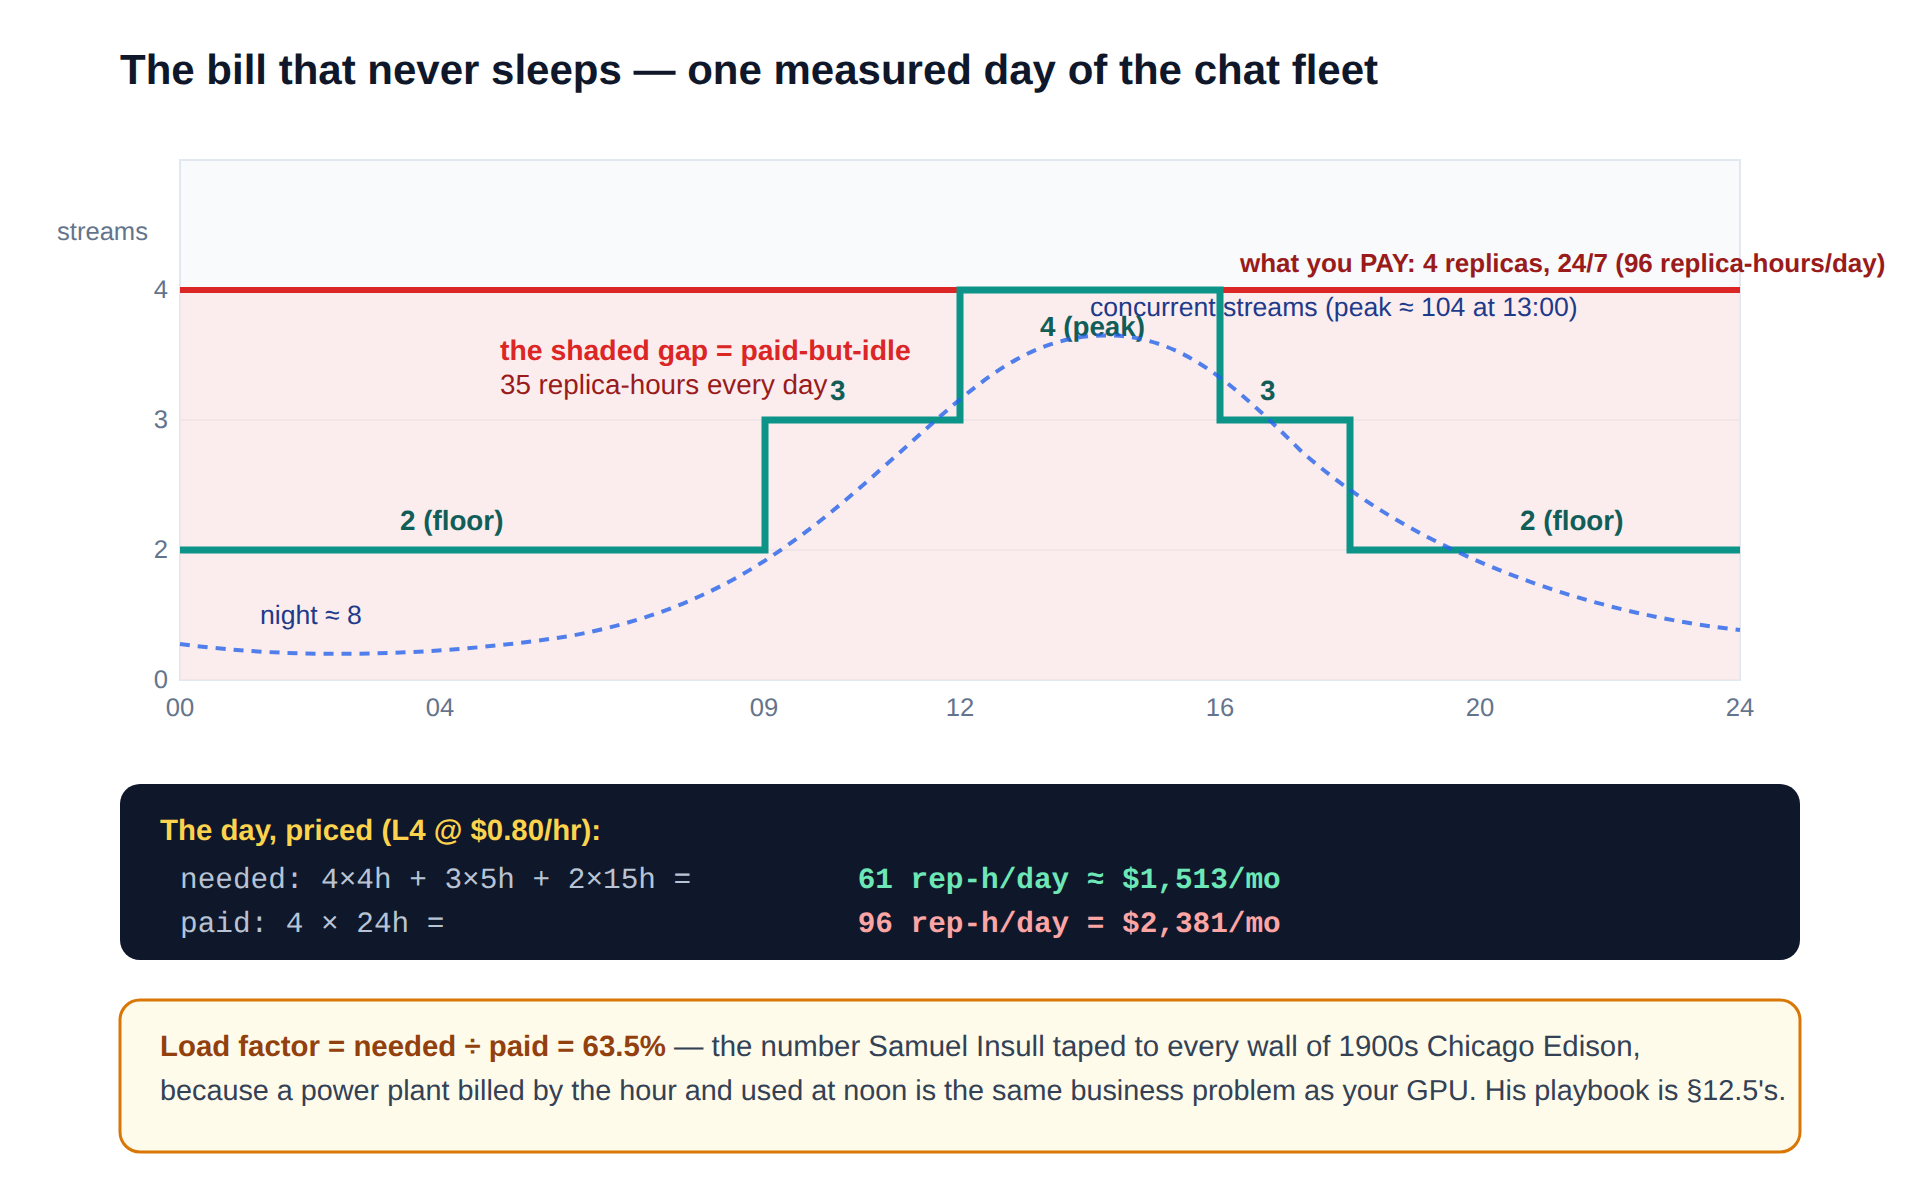
\includegraphics{figures/fig12-1_diurnal.png}}\\[3pt]
  \figcaption{Figure 12-1  The day, drawn. The staircase is what the SLO actually requires (with a floor of two for rollout safety); the flat red line is what a static fleet pays. The gap is 35 replica-hours of night shift, every day, \$868 a month.}
\end{tbbfigure}

\subsection*{1902: the last industry to face this exact bill}

Here is the consoling news: this is not a new problem, and the industry that solved it did so before your grandparents were born — selling not GPU-hours but kilowatt-hours. Around 1900, electricity companies were going broke on precisely Exhibit 12-A's arithmetic: a power plant is a massive fixed cost that is \textit{sized for the evening lighting peak} and sits underused the other twenty hours. \textbf{Samuel Insull} — Thomas Edison's former secretary, by then running Chicago's electric utility — became obsessed with one metric, and it was not revenue: it was \textbf{load factor}, average demand over peak demand, the exact ratio at the bottom of Exhibit 12-A. His insight was that a utility's true product is \textit{capacity}, and idle capacity is pure loss; the game is to fill the valleys and shave the peaks. So his company pioneered the whole playbook: \textbf{metering demand, not just consumption} (your peak sets the plant size, so your peak should set your bill — cloud pricing's ancestor); \textbf{courting customers whose peaks interlocked} — streetcars by day, lighting by evening, ice plants and factories overnight — so one plant served three demand curves; \textbf{selling off-peak power cheap} to anyone who could shift their work into the valley; and \textbf{interruptible rates} for industrial customers willing to be shed at peak. Electricity went from a luxury priced around twenty cents a kilowatt-hour toward a couple of cents within two decades — not mainly through better dynamos, but through better \textit{load factor}. Every mechanism in this chapter — autoscaling, scale-to-zero, GPU sharing, spot instances, the night-batch trick — is one of Insull's moves wearing a Kubernetes T-shirt, and §12.5 will buy capacity exactly the way his customers bought power.

\subsection*{The obvious fix meets two ambushes}

"Just change the replica count with demand" is, mechanically, almost insultingly easy — Chapter 5 promised as much: an autoscaler is \textit{another writer of desired state}, editing one integer while controllers do everything else. The interesting engineering is in the two ways the easy version fails, and Exhibit 12-B stages them both:

\begin{terminalbox}
\begin{Verbatim}[breaklines=true,breakanywhere=true,fontsize=\small,formatcom=\color{tbbtermfg},codes=\tbbcodeactive]
# attempt 1, monday: the tutorial default.
$ kubectl autoscale deploy/chat --cpu-percent=70 --min=2 --max=6
$ kubectl get hpa chat -w              # tuesday, 09:00 wave arrives
NAME   REFERENCE     TARGETS       MINPODS  MAXPODS  REPLICAS
chat   deploy/chat   cpu: 9%/70%      2        6        2
# GPUs drowning (queue growing, TTFT p99 6.1s). CPU: napping at 9%.
# verdict: "9% < 70%, all quiet." it will NEVER scale. wrong eye.

# attempt 2, wednesday: right metric (KEDA on the vLLM queue).
09:00:15  waiting=41 -> desired 2->4       # right eye reacts in 15 s
09:00:24  2 pods Pending -> Init -> ...
09:02:54  ...Ready                         # cold start: 2.5 minutes
# 09:00-09:03: TTFT p99 red. right metric, LATE muscle.
# lesson 1: scale on what users feel. lesson 2: reaction time
# is part of capacity. the wave does not wait for your pods.
\end{Verbatim}
\end{terminalbox}
\figcaption{Exhibit 12-B  Two failures, one morning each. The CPU-based autoscaler never fires (the GPU's busyness is invisible to it); the queue-based one fires in fifteen seconds and then spends two and a half minutes giving birth. §12.2 fixes the eye; §12.3 fixes the stopwatch.}

Those two ambushes give the chapter its spine. \textbf{§12.2} wires the autoscaler to the metric Chapter 11 taught you to read — the admission queue — and works the control loop's real knobs: the desire formula, the asymmetric stabilization windows, the scheduled ramp for the peak you can predict. \textbf{§12.3} itemizes the 2.5-minute birth — image, weights, engine, warm-up, and the Week 2 Firecracker callback that explains which line item the industry already solved — then climbs the mitigation ladder, ending at scale-to-zero and its honest niche. \textbf{§12.4} attacks the \textit{other} waste Exhibit 1-B exposed — services too small for their whole GPU — by bending Chapter 2's one-tenant-per-card rule: time-slicing, MPS, MIG. \textbf{§12.5} assembles Insull's portfolio in cloud pricing (committed floor, on-demand shoulder, spot burst, off-peak fill), walks the project's bill from \$2,381 to \textbf{\$877 — under the Week 1 ceiling, with receipts} — and closes Chapter 1's build-vs-buy break-even with measured unit economics. \textbf{§12.6} is the lab the syllabus has been building toward: the team project's midpoint review, where every number you present traces to a sweep or a price sheet.

\begin{calloutbox}{tbbpurple}{tbbpurplefill}
{\normalsize\bfseries\color{tbbpurple}Think About It}\par\vspace{3pt}
\begin{tbbitemize}
  \item Exhibit 12-A's floor is 2 replicas, justified as "rollout safety." Reconstruct the argument from Chapter 5's rolling-update mechanics (maxUnavailable/maxSurge) and Chapter 11's streams — then argue the OTHER side: what would have to be true of your traffic and your users for a floor of 1, or 0, to be defensible?
  \item Insull's demand meter billed customers on their PEAK, not their total consumption. Map that onto cloud GPU pricing: what is the cloud's equivalent of a demand charge, and why does the hourly on-demand price already encode Insull's logic? (Hint: who bears the idle risk in each pricing model?)
  \item Exhibit 12-B's attempt 1 would actually scale — under one traffic pattern. Describe it, explain why a GPU chat service will never produce it, and name the Chapter 9 exhibit this is the mirror image of.
  \item A teammate proposes fixing the 09:00 ambush with max=6 and a permanently lower target ("more headroom all day"). Price that proposal against Exhibit 12-A's ledger, and name what it actually buys (hint: it re-flattens the staircase).
\end{tbbitemize}
\end{calloutbox}

\section{Autoscaling: The Right Metric and the Stopwatch}

Strip the mystique first, because Chapter 5 already did the hard part. A \textbf{Horizontal Pod Autoscaler} is a control loop that, every fifteen seconds, reads a metric, computes how many replicas \textit{would} bring that metric to a target, and writes the answer into the Deployment's \code{replicas} field. That is the entire machine: \textbf{observe → desire → edit one integer}. Everything downstream — scheduling, image pulls, weight loads, probes, Service membership — is Chapter 5's reconciliation machinery keeping a promise it has kept since Week 5; the §5.2 think-box asked you to notice "how little the autoscaler itself has to know," and here is the payoff. The desire arithmetic is one line: \textbf{desired = ceil(current × metric ÷ target)}. Two replicas carrying 41 waiting requests against a target of 10-per-replica: desired = ceil(2 × 20.5 ÷ 10) = \textbf{5}, capped by \code{maxReplicas: 4}. No machine learning, no forecasting — a thermostat, not a meteorologist. The engineering content lives in two questions the formula takes as given: \textit{which metric}, and \textit{how fast the new capacity actually arrives}.

\begin{tbbfigure}
  \adjustbox{max width=0.94\linewidth,max totalheight=0.46\textheight}{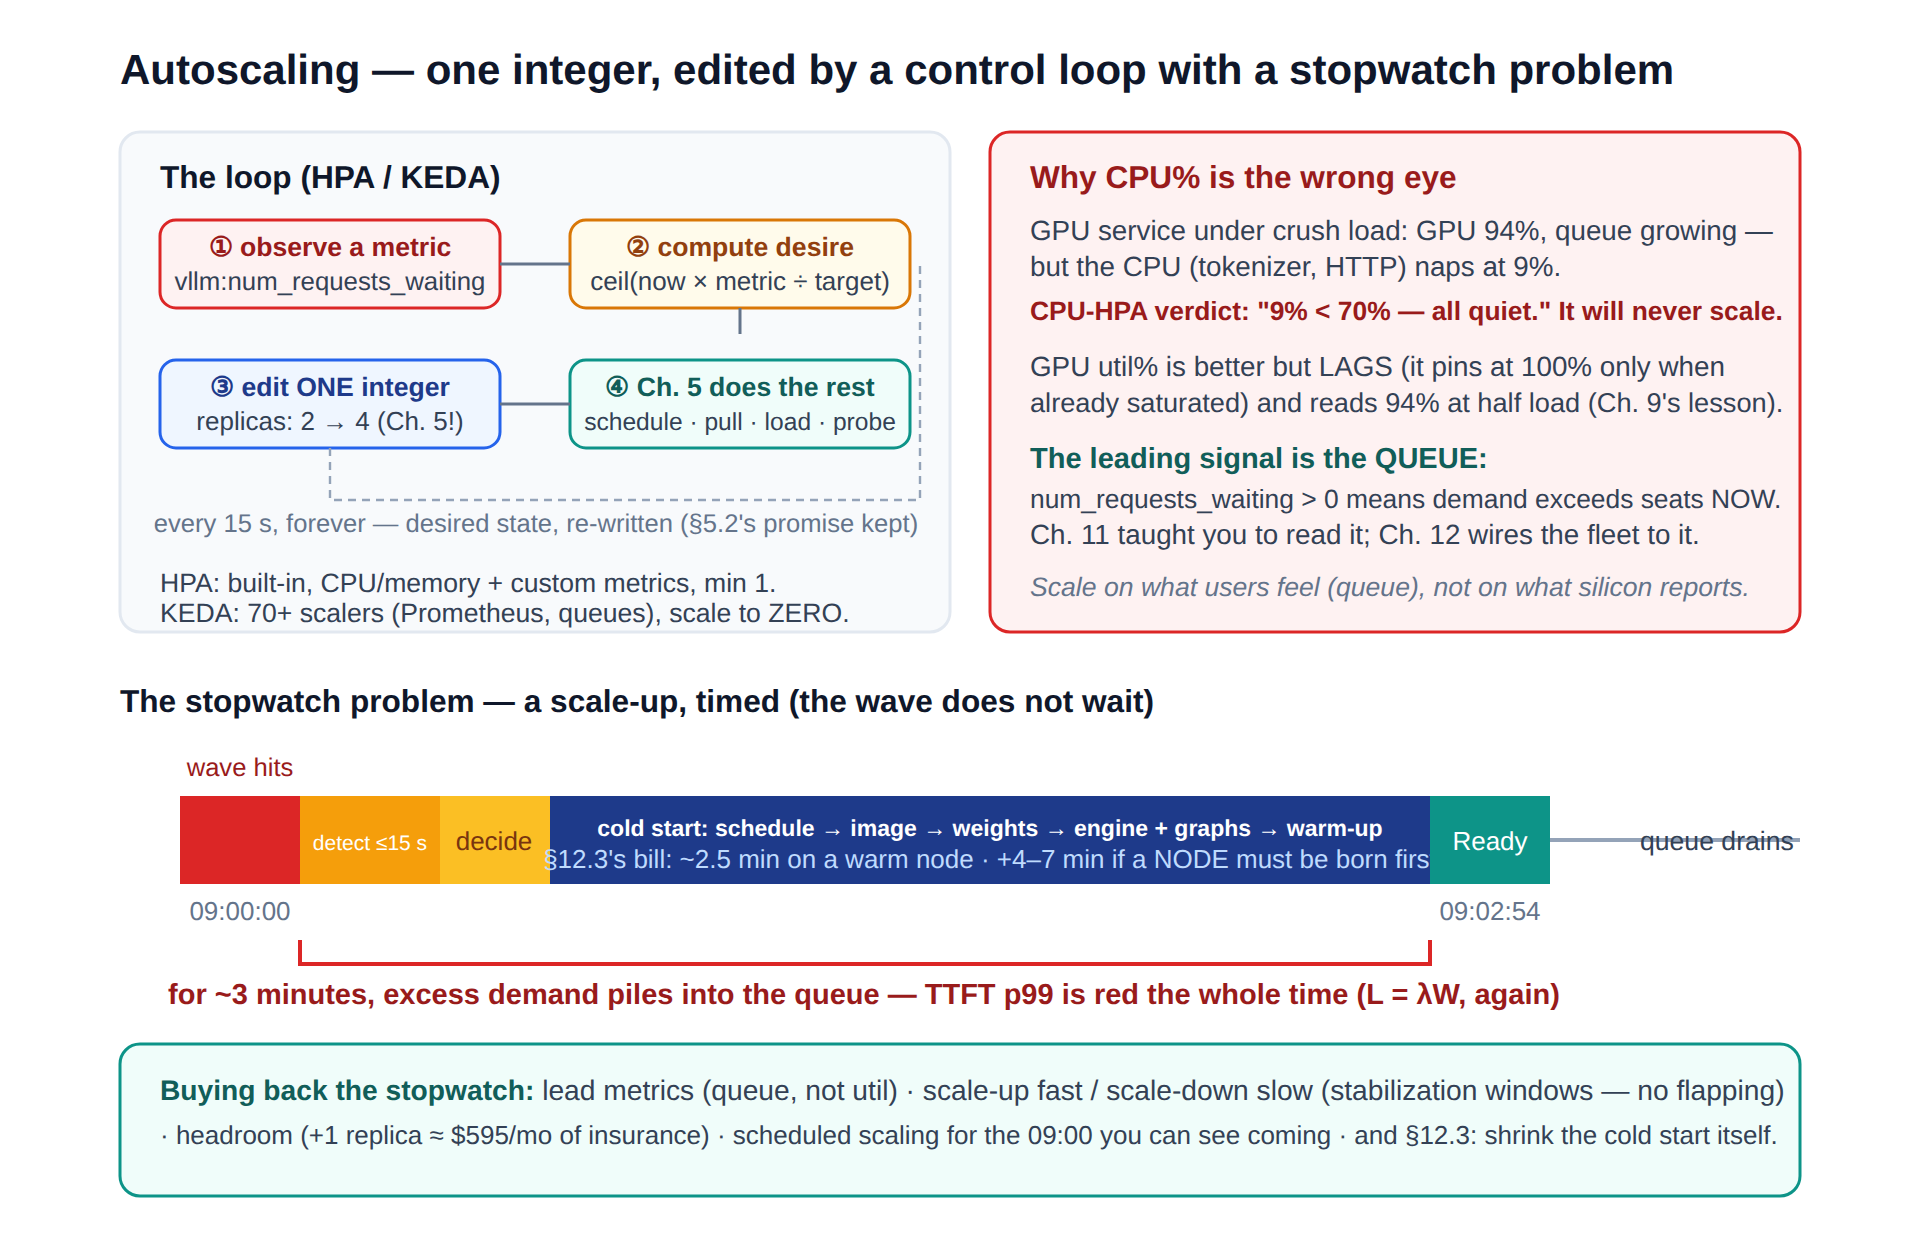
\includegraphics{figures/fig12-2_autoscale.png}}\\[3pt]
  \figcaption{Figure 12-2  The loop and its two failure modes. Left: the four-beat cycle, editing desired state. Right: why CPU\% never fires for a GPU service. Bottom: the stopwatch — detection is seconds, birth is minutes, and the queue eats the difference.}
\end{tbbfigure}

\subsection*{The eye: scale on what users feel}

Exhibit 12-B's Monday failure is worth dissecting because its logic error is \textit{invisible} on every dashboard. The default HPA watches \textbf{CPU\%} because for a fleet of web servers CPU genuinely is the contended resource. Your chat service inverts the anatomy — Chapter 9's Exhibit A showed a CPU pinned at 100\% while the GPU idled at 7\%; the GPU service under load is the mirror image: GPU at 94\%, tokenizer-and-HTTP CPU sipping 9\%, and the CPU-eyed autoscaler concluding \textit{all quiet} while the queue grows without bound. \textbf{GPU utilization\%} is the tempting second choice and still the wrong one, twice over: it \textit{saturates} (once the card reads \textasciitilde{}100\% it cannot express "and demand is 3× beyond that," so the autoscaler undershoots exactly when the gap is largest), and it \textit{lies at partial load} (Chapter 9 taught you a kernel-launch-bound service can read 90\%+ while serving half its capacity). The correct eye is the one Chapter 11 built into the engine: \textbf{vllm:num\_requests\_waiting} — the admission queue. It is a \textit{leading} indicator (nonzero the instant demand exceeds seats, before any latency percentile moves), it is \textit{unbounded} (41 waiting says exactly how wrong capacity is), and it is \textit{what users feel} (the queue is TTFT's numerator, by L = λW). The general rule, worth a margin note in every runbook you ever write: \textbf{scale on demand signals (queue depth, in-flight concurrency), not on supply-side gauges (CPU\%, GPU\%, memory)} — gauges tell you how hard the machine works, queues tell you how long users wait, and the SLO is written about users.

Mechanically, custom metrics reach the autoscaler by one of two roads. The \textbf{HPA road}: install a metrics adapter (prometheus-adapter) that translates PromQL into the Kubernetes custom-metrics API — powerful, fiddly, and min-replicas stops at 1. The \textbf{KEDA road}, which the lab takes: KEDA is an operator with seventy-plus \textit{scalers} (Prometheus, SQS, Kafka, cron...) that manages an HPA for you from one CRD — and it can scale \textbf{to zero}, which the HPA cannot (§12.3 explains why zero is a different beast). One \code{ScaledObject} says everything this section has argued:

\begin{terminalbox}
\begin{Verbatim}[breaklines=true,breakanywhere=true,fontsize=\small,formatcom=\color{tbbtermfg},codes=\tbbcodeactive]
apiVersion: keda.sh/v1alpha1
kind: ScaledObject
metadata: {name: chat-scaler}
spec:
  scaleTargetRef: {name: chat}          # the Deployment to edit
  minReplicaCount: 2                    # the floor (rollout safety)
  maxReplicaCount: 4                    # the budget ceiling
  cooldownPeriod: 300                   # scale DOWN slowly (5 min)
  triggers:
  - type: prometheus
    metadata:
      serverAddress: http://prometheus:9090
      query: sum(vllm:num_requests_waiting{app="chat"})
      threshold: "10"                   # tolerate 10 waiting/replica
# scale on the queue users feel - not the CPU nobody uses.
\end{Verbatim}
\end{terminalbox}
\figcaption{Transcript 12-1  The lab's ScaledObject. Fifteen lines encode the section: the right metric (the vLLM admission queue), a floor for safety, a ceiling for budget, and an asymmetric temper — eager up, reluctant down.}

\subsection*{The temper: eager up, reluctant down}

The formula alone would produce a nervous fleet — traffic wobbles, and a scaler that mirrors every wobble \textbf{flaps}: replicas appear, pay their 2.5-minute birth, serve eight minutes, die, and are re-born for the next wobble, converting your bill into pure cold-start overhead. (You met flapping's nastiest special case in a Chapter 10 think-box: every scale-out pod paying a 40-second torch.compile warm-up on arrival, p99 spiking on each one.) The industry's cure is \textbf{asymmetric stabilization}: scale \textbf{up} on the instantaneous signal (a real queue must never wait for smoothing — seconds matter), scale \textbf{down} only on the \textit{worst case over a trailing window} (HPA behavior: \code{scaleDown.stabilizationWindowSeconds: 300}; KEDA: \code{cooldownPeriod}). The asymmetry encodes an asymmetric loss function you can defend to a CFO: scaling up too eagerly wastes a few replica-minutes; scaling down too eagerly breaks the SLO you spent five chapters measuring. Set the down-window from your traffic's wobble period (five minutes suits diurnal chat; batchy traffic wants more), and set the \textbf{floor} from operations, not load: two replicas lets Chapter 5's rolling update retire one while the other serves — a floor of one turns every deploy into a brownout.

\subsection*{The stopwatch: reaction time is part of capacity}

Now the Wednesday ambush. Even with the right eye and a calm temper, the loop's end-to-end reaction time is \textbf{T = detect (≤15 s metric scrape) + decide (≤15 s loop tick) + provision (§12.3's cold start: \textasciitilde{}150 s pod-on-warm-node, 6–10 min if a GPU node must be born)} — call it three minutes for the honest case. During those minutes the \textit{old} fleet absorbs the \textit{new} demand, and the queue integrates the difference: the 09:00 wave lifts offered load from 64 to 104 concurrent streams against 64 seats, so \textasciitilde{}9 turn-arrivals per second find no seat, and by Ready-time roughly forty streams' worth of demand has pooled in the queue — which is precisely Transcript 11-3's regime 3, TTFT p99 red, reproduced on a schedule every morning. Three remedies, in the order you should reach for them. \textbf{Scheduled scaling} for peaks you can see coming: traffic that ramps every weekday at 09:00 is not a prediction problem, it is a calendar problem — a KEDA cron trigger raising the floor to 4 at 08:40 deletes the ambush for the price of 40 minutes × 2 replicas ≈ \textbf{\$1.07 a day}. \textbf{Headroom} for peaks you cannot: running the target slightly rich (tolerate 5 waiting instead of 10) or holding +1 replica through business hours (\textasciitilde{}\$50/mo) buys the queue time to survive detection+birth. \textbf{Shrink the birth itself} — which is the next section entire. What does \textit{not} work is wishing the loop faster: one-second scrape intervals against a 150-second birth just measure the ambush more precisely.

\begin{terminalbox}
\begin{Verbatim}[breaklines=true,breakanywhere=true,fontsize=\small,formatcom=\color{tbbtermfg},codes=\tbbcodeactive]
# wednesday again, with the 08:40 cron floor + KEDA queue trigger:
$ kubectl get hpa keda-hpa-chat-scaler -w
TIME      TARGETS        REPLICAS   EVENT
08:40:02  0/10 (cron:4)  2 -> 4     # calendar, not clairvoyance
08:42:33  0/10           4          # 2 births paid BEFORE the wave
09:00:00  wave arrives: streams 64 -> 104
09:00:15  3/10           4          # queue: single digits. absorbed.
09:14:00  peak passes; waiting=0 for 5 min (cooldown)...
09:19:05  0/10           4 -> 3     # reluctant down. no flapping.
# TTFT p99 through the whole event: 0.46 s. the ambush is deleted -
# for $1.07 of pre-warm. compare Exhibit 12-B's three red minutes.
\end{Verbatim}
\end{terminalbox}
\figcaption{Transcript 12-2  The wave, survived. A cron trigger pays two births before the peak; the queue trigger handles the shape; the cooldown keeps the descent calm. The SLO holds through the event for about a dollar — the cheapest insurance this course sells.}

One boundary honesty note: everything above scales \textbf{pods within a provisioned node pool}. When desired pods exceed node capacity, the \textbf{cluster autoscaler} must birth a GPU \textit{machine} — 3–7 minutes of capacity hunt, boot, and driver install, occasionally ending in "no capacity in zone" (GPU scarcity is real weather; Chapter 2's quota lab was the gentle preview). The operational rule falls out of the numbers: \textbf{pods chase waves; nodes follow forecasts.} Pre-provision the day's node envelope (the staircase's maximum), let pod-autoscaling breathe inside it, and treat node-autoscaling as a slow daily tide — never as the thing standing between a 09:00 wave and your TTFT clause.

\begin{calloutbox}{tbbpurple}{tbbpurplefill}
{\normalsize\bfseries\color{tbbpurple}Think About It}\par\vspace{3pt}
\begin{tbbitemize}
  \item Run the desire formula through Transcript 11-3's regime 3 (running 32, waiting 26, one replica, target 10): what does the HPA ask for, what does maxReplicas cap it to, and — using §11.3's seat arithmetic — is the cap right? What budget number would justify raising it?
  \item Your traffic has two peak shapes: the predictable 09:00 ramp and unpredictable social-media spikes (3× in 90 seconds, gone in 10 minutes). Design the trigger set (cron + queue + headroom) for both, and state which spike the design deliberately sacrifices, and why that is the correct CFO conversation.
  \item A teammate sets scaleDown stabilization to 30 s "to save money faster." Model one hour of wobbly traffic (peaks every \textasciitilde{}7 min): count births, price the cold-start overhead at 150 s each, and show the "saving" is negative — then find the traffic pattern where they would be right.
  \item Defend the floor-of-2 to a cost reviewer using only Chapter 5 vocabulary (rolling update, maxUnavailable, probe gating) — then compute what the floor costs per month and what single product decision would let it drop to 1.
\end{tbbitemize}
\end{calloutbox}

\section{Cold Starts and Scale-to-Zero}

The autoscaler's muscle is only as fast as a replica's birth, so this section does to the cold start what Chapter 7 did to latency: \textbf{stops treating it as a number and itemizes it as a bill}. You have been assembling the line items for nine chapters — Chapter 4 priced the image pull, Chapter 6 built the weight-loading bar and warned "Week 12 fights over this bar," Chapter 10 priced runtime compilation, Chapter 11 added the engine's KV-pool allocation and CUDA-graph capture. Watch one pod pay all of them at once:

\begin{terminalbox}
\begin{Verbatim}[breaklines=true,breakanywhere=true,fontsize=\small,formatcom=\color{tbbtermfg},codes=\tbbcodeactive]
$ kubectl describe pod chat-7f9b4-x2kkj | grep -A2 Events; kubectl logs -f ...
09:00:24  Scheduled    assigned to node gpu-pool-b7   #     +2 s
09:00:26  Pulling      image "registry/chat:v9"
09:00:42  Pulled       3.1 GB in 16.1 s               # Ch. 4's slim image,
                                                      # warm node layer cache
09:00:44  vllm  INFO   Fetching weights: 16-way ranged GET
09:00:53  vllm  INFO   6.02 GiB in 8.9 s              # Ch. 6's loader
09:02:28  vllm  INFO   engine init: VRAM load, KV pool alloc,
                       CUDA graph capture... 95 s     # Ch. 11's engine
09:02:54  Ready        readiness probe passed          # after 26 s of
                                                      # scripted warm-up
# total: 150 s. the pod path. if a NODE had to be born first:
# +3-7 min (VM provision, boot, driver install) - and sometimes
# "no capacity in zone." never put a node birth on the SLO path.
\end{Verbatim}
\end{terminalbox}
\figcaption{Transcript 12-3  One birth, itemized. Every line has a chapter: the 16-second pull is Chapter 4's engineering, the 9-second weight fetch is Chapter 6's, the 95-second engine init is Chapter 11's — and the sum, 150 seconds, is §12.2's stopwatch problem quantified.}

\begin{tbbfigure}
  \adjustbox{max width=0.94\linewidth,max totalheight=0.46\textheight}{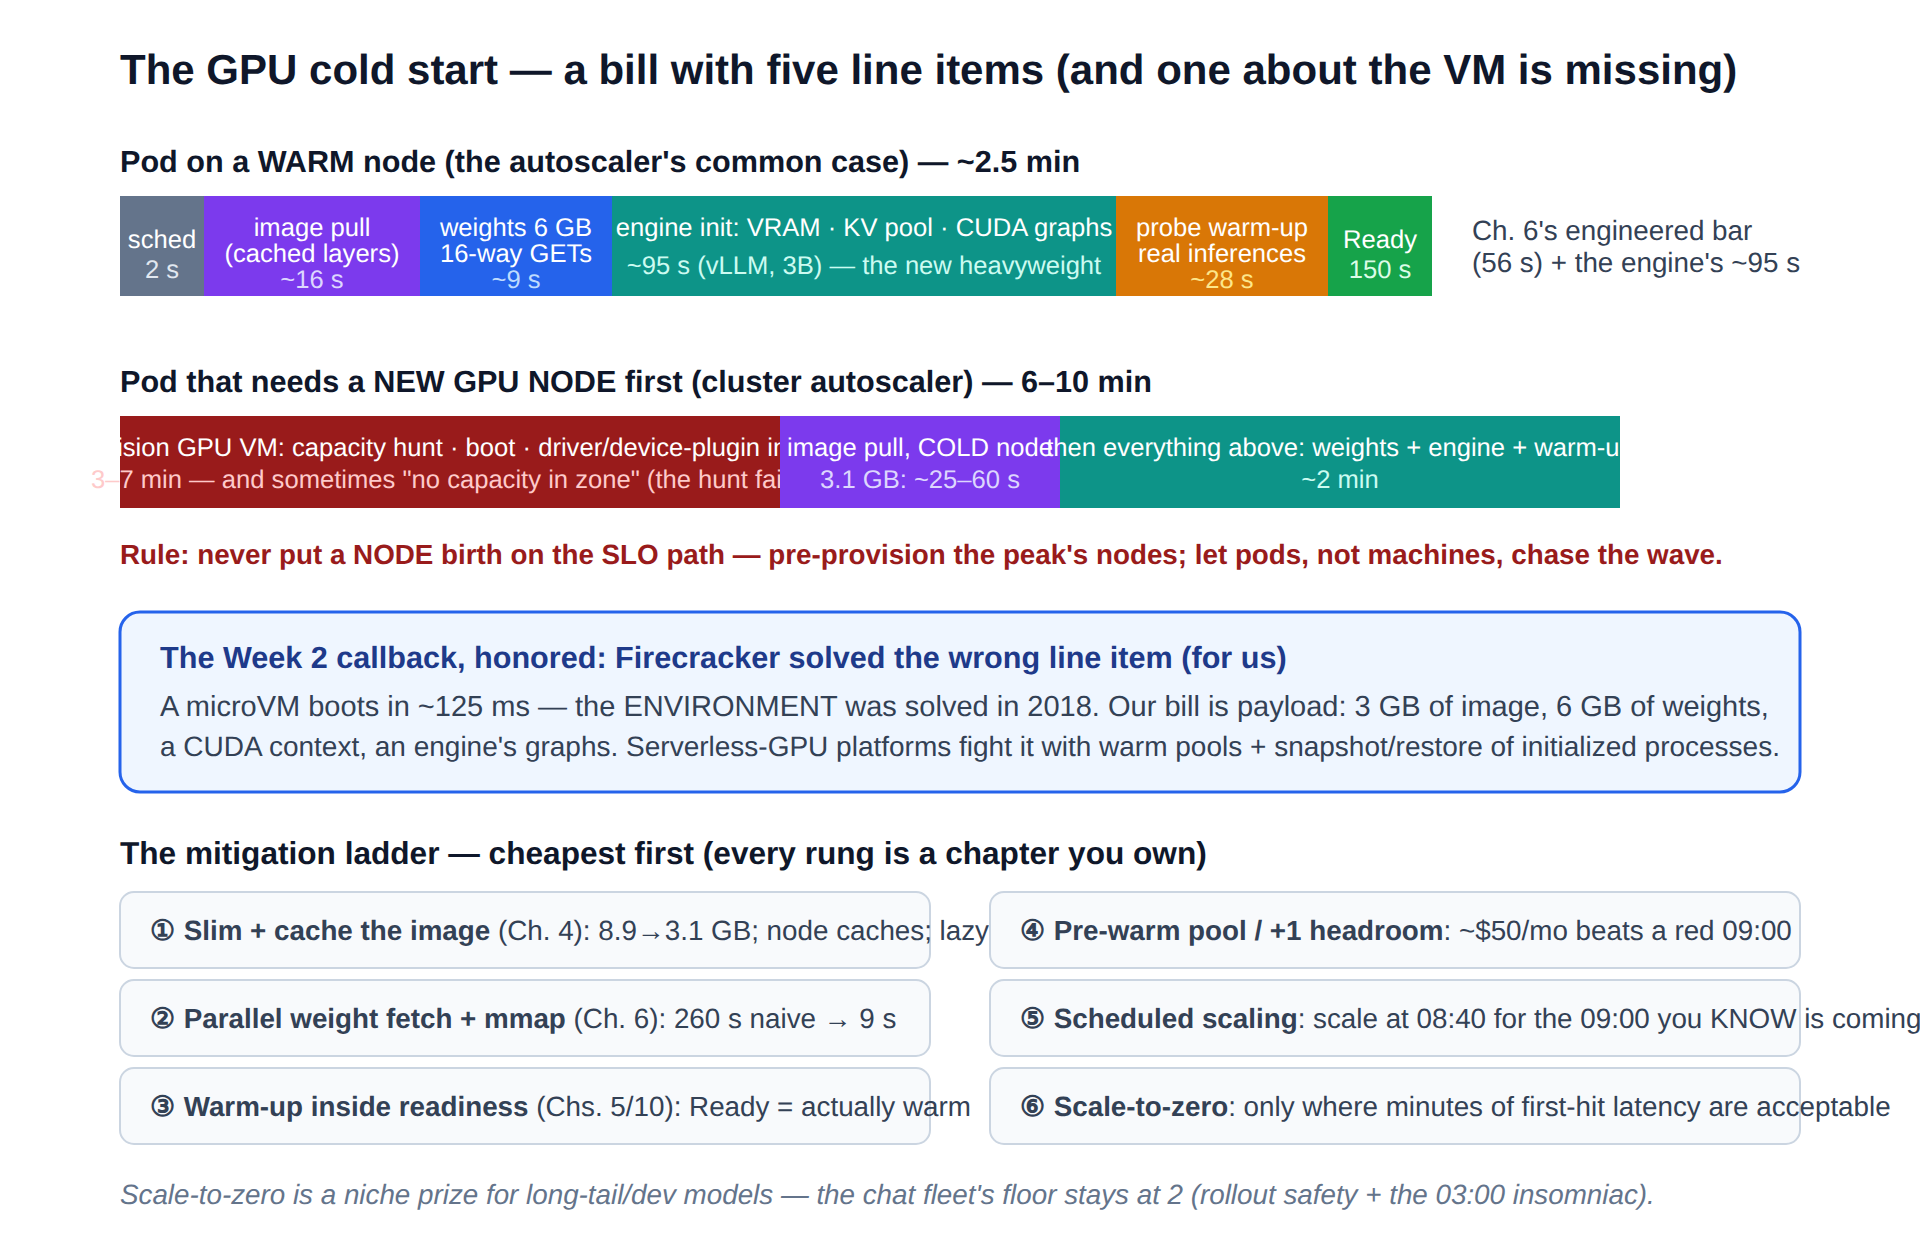
\includegraphics{figures/fig12-3_coldstart.png}}\\[3pt]
  \figcaption{Figure 12-3  The bill, both paths, and the ladder. The warm-node pod costs \textasciitilde{}2.5 minutes, dominated now by engine initialization; the node path multiplies it; and each mitigation rung is a chapter this course already taught.}
\end{tbbfigure}

\subsection*{The Firecracker callback — solved, but the wrong line item}

Week 2 planted a promise this section must now keep. Firecracker's microVM boots in \textbf{\textasciitilde{}125 milliseconds} — the isolation environment that took minutes in 2005 became effectively free by 2018, and Chapter 2's §2.4 told you its Week 12 lesson in advance: \textit{"the environment stopped being the bottleneck; the payload is."} Read Transcript 12-3 against that claim: the VM/container machinery contributes the two-second \code{Scheduled} line and essentially nothing else. The 148 remaining seconds are \textbf{payload} — 3.1 GB of image, 6 GB of weights, a CUDA context, an engine's worth of allocations and graph captures. This is why "serverless GPU" is genuinely hard where serverless CPU was merely clever: Lambda's trick (pools of pre-booted microVMs + snapshot/restore) attacks a millisecond-scale problem; the GPU version must pre-position \textit{gigabytes} and re-hydrate an initialized CUDA process. The platforms that sell per-second GPU billing (Modal, RunPod, Cloud Run GPU) fight exactly this war — warm pools, aggressive image streaming, and increasingly \textbf{GPU checkpoint/restore} (snapshot a fully-initialized engine process, restore it in seconds; the "sub-second cold start" engineering posts in this chapter's further reading are all variations) — and their pricing tells you the war is not free: per-second rates carry a premium over the raw VM. The course fleet does not need them; it needs the ladder.

\subsection*{The mitigation ladder — and the honest niche of zero}

Climb Figure 12-3's ladder cheapest-first, and notice you already own every rung. \textbf{① Image hygiene} (Ch. 4): the multi-stage 3.1 GB image with warm node caches took 16 s where the naive 8.9 GB took a minute; lazy-pull snapshotters (eStargz, image streaming) start the container before the image finishes arriving. \textbf{② Weight logistics} (Ch. 6): 16-way ranged GETs + safetensors mmap turned 260 s into 9; a node-local cache turns the \textit{second} birth on a node into a disk read. \textbf{③ Warm-up inside readiness} (Chs. 5/10): the probe runs scripted inferences so \code{Ready} means \textit{warm} — this line item is unavoidable work, but gating it correctly means the LB never routes to a cold pod (and the Ch. 10 flapping story cannot recur). \textbf{④ Pre-warm headroom} (§12.2): +1 replica through business hours, \textasciitilde{}\$50/mo, converts birth latency into money at a known exchange rate. \textbf{⑤ Scheduled scaling}: the 08:40 cron — birth paid before demand exists. \textbf{⑥ Scale-to-zero}: the far rung, and a different animal, because the \textit{first} request after zero eats the entire 150 s (or the node path's minutes) as user-visible latency. KEDA can do it (its HTTP add-on parks requests while the birth runs); Knative made it a religion; and the honest decision rule is one sentence: \textbf{scale-to-zero is for endpoints whose callers can absorb minutes of first-hit latency} — the long-tail internal model used twice a week (\$595/mo of idle L4 → \textasciitilde{}\$3), the dev environment, the batch-triggered scorer. The chat fleet's floor stays at 2: the 03:00 insomniac is a paying user, and Chapter 5's rollouts need a partner. Run the arithmetic per endpoint and the fleet sorts itself: \textbf{zero for the long tail, floors for the SLO-bearing head.}

\begin{calloutbox}{tbbpurple}{tbbpurplefill}
{\normalsize\bfseries\color{tbbpurple}Think About It}\par\vspace{3pt}
\begin{tbbitemize}
  \item Transcript 12-3's engine init (95 s) is now the dominant line. Using Chapters 10–11: which parts of it scale with model size, which with KV-pool size, and which are fixed? Propose the two most promising attacks (hint: AWQ weights are 1.9 GB; CUDA-graph capture can be narrowed) and estimate each one's savings.
  \item Price scale-to-zero for three endpoints: (a) the chat fleet, (b) a nightly batch scorer, (c) an internal RAG demo used \textasciitilde{}5×/week. For each: idle-\$ saved, first-hit latency cost, and the verdict — then name the product sentence that would flip verdict (a).
  \item A "sub-second GPU cold start" blog post makes the rounds. From this section, list what must be true behind that headline (what was snapshotted? where do weights live? who pays for the warm pool?) — and what the benchmark almost certainly does NOT include.
  \item Your cluster autoscaler occasionally reports "no capacity in zone" for L4s at peak. Design the fallback chain (other zone → other GPU type → on-demand→spot inversion → queue-and-degrade) and mark which steps Chapter 5's nodeSelector/affinity machinery can express today.
\end{tbbitemize}
\end{calloutbox}

\section{Sharing the Silicon: Time-Slicing, MPS, MIG}

Autoscaling repairs the waste of \textit{too many whole GPUs}; this section repairs the opposite embarrassment, and it is the one Chapter 1 opened the course with: \textbf{Exhibit 1-B's ghost} — an A10G billed \$779.66 for a month of 0.2\% utilization, a whole card owned by a service too small to use it. Chapter 2 §2.6 explained \textit{why} the waste was structural: GPUs resist virtualization (no VT-x equivalent, kernel can't preempt driver-queued work), so the cloud's unit of rental became \textbf{one tenant, one card} — passthrough's clean isolation at passthrough's brutal granularity. It also promised that Week 12 would bend the rule three ways. Here are the three ways, ordered by how much isolation they surrender for how much utilization they recover.

\begin{tbbfigure}
  \adjustbox{max width=0.94\linewidth,max totalheight=0.46\textheight}{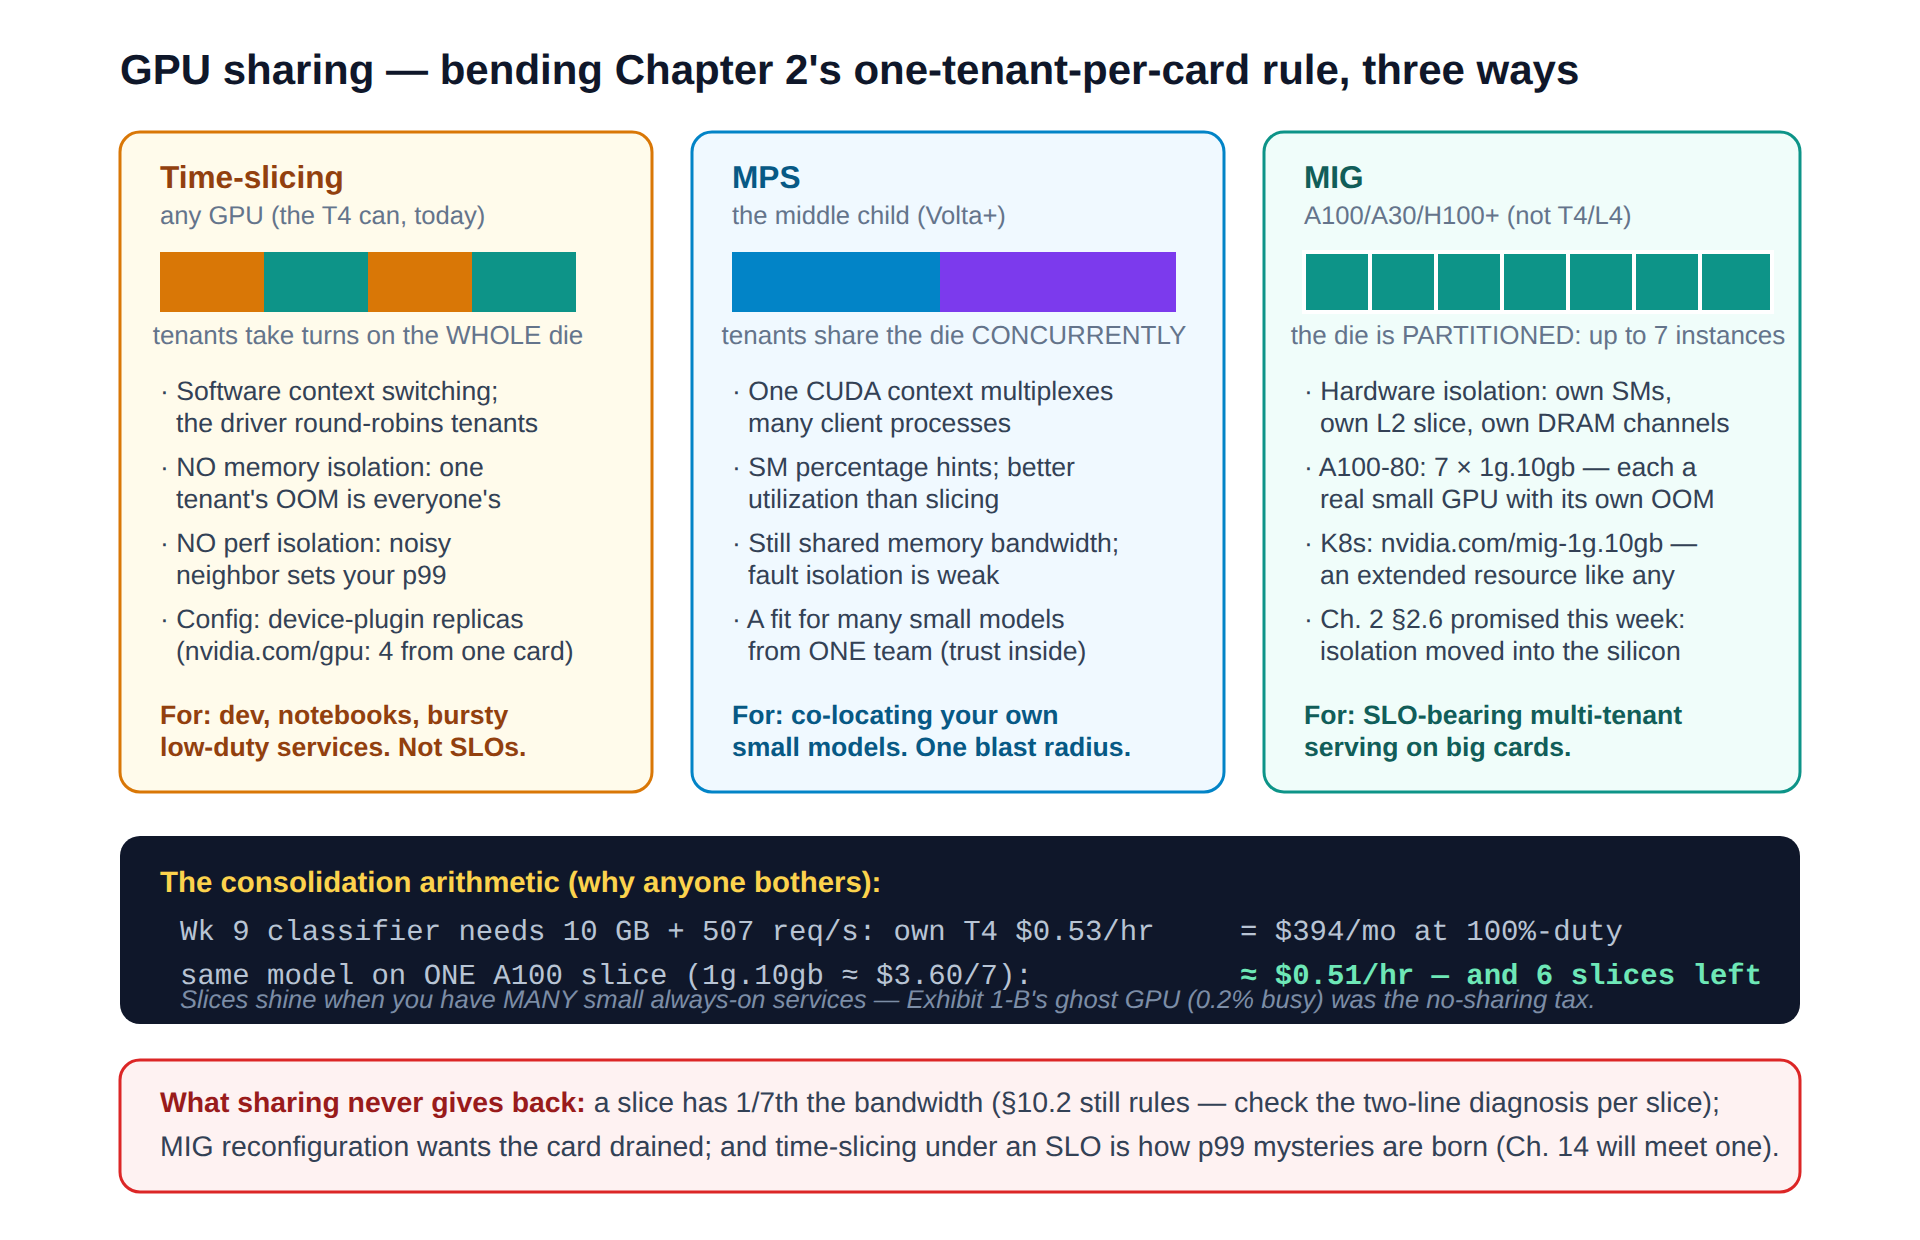
\includegraphics{figures/fig12-4_sharing.png}}\\[3pt]
  \figcaption{Figure 12-4  The sharing spectrum. Time-slicing: take turns on the whole die (no isolation). MPS: share the die concurrently (one blast radius). MIG: partition the die in hardware (real walls, coarse granularity) — Chapter 2's rule, bent by the silicon itself.}
\end{tbbfigure}

\subsection*{Time-slicing: taking turns, honestly labeled}

\textbf{Time-slicing} is the bluntest bend: the driver context-switches the \textit{whole GPU} among tenants, a few milliseconds each, exactly as a 1970s time-sharing OS shared one CPU. Kubernetes wires it through the device plugin's config — advertise \code{replicas: 4} and one physical card presents as \code{nvidia.com/\allowbreak gpu: 4}, schedulable by four pods that each believe they own it. What it buys: any GPU works (the lab's T4 included), setup is one ConfigMap, and four 10\%-duty services stop wasting 3.6 cards. What it surrenders — and the lab makes you \textit{measure} — is everything Chapter 2 valued about passthrough: \textbf{no memory isolation} (VRAM is first-come-first-served; one tenant's leak OOMs its neighbors — Exhibit 11-B's creep, now a \textit{shared} creep), \textbf{no performance isolation} (your p99 now contains your neighbor's batch sizes; the context switches themselves tax every tenant), and \textbf{no fault isolation} (one Xid error resets everyone's afternoon). The honest use cases write themselves: dev boxes, notebooks, interactive experiments, and low-duty \textit{internal} services where the neighbors are all you. Under a customer-facing SLO, time-slicing is how Chapter 14's unexplainable-p99 war stories get written.

\begin{terminalbox}
\begin{Verbatim}[breaklines=true,breakanywhere=true,fontsize=\small,formatcom=\color{tbbtermfg},codes=\tbbcodeactive]
# lab part A-④: slice the T4 four ways, then MEASURE the rent.
$ kubectl apply -f timeslice-config.yaml   # device-plugin: replicas: 4
$ kubectl describe node gpu-node | grep nvidia.com/gpu
  nvidia.com/gpu:  4        # one card, four schedulable "GPUs"
$ kubectl scale deploy/clf --replicas=2    # two classifiers co-tenant

# same sweep as Week 9, alone vs. with a busy neighbor:
            p50      p99      req/s@SLO
alone      2.9ms    9.8ms      507
neighbor   3.1ms   38.4ms      214       # p99 x3.9, capacity /2.4
# nothing is "broken." the card is just honest: two tenants, one die.
# noisy neighbor is not folklore - it is a number you now own.
\end{Verbatim}
\end{terminalbox}
\figcaption{Transcript 12-4  Sharing, measured. Two classifier pods time-slice the lab T4; each alone is fine, together the p99 quadruples — the isolation Chapter 2 said passthrough bought, visible in its absence. Sharing is a real discount with a real price tag.}

\subsection*{MPS and MIG: the middle, and the hardware answer}

\textbf{MPS} (Multi-Process Service) is the middle rung: instead of taking turns, tenant processes' kernels run \textbf{concurrently} through one shared CUDA context, with optional per-client SM-percentage caps. Utilization beats slicing (no context-switch tax; idle SMs genuinely absorb neighbor work), and Volta+ added address-space isolation — but memory bandwidth is still communal, and the blast radius is still shared, which is why MPS's sweet spot is \textbf{many small models from one team}: you are your own noisy neighbor, and you can negotiate with yourself. \textbf{MIG} is the answer Chapter 2 §2.6 promised: from Ampere on, the big dies (A100, A30, H100 — \textit{not} the lab's T4 or the fleet's L4) partition \textbf{in hardware} into up to seven instances, each owning its own SM slice, L2 slice, and DRAM controllers. A MIG slice is a real small GPU: its own OOM, its own faults, bandwidth that is \textit{provisioned} rather than contended — isolation moved into the silicon, the exact phrase the chapter used. Kubernetes sees each profile as an extended resource (\code{nvidia.com/\allowbreak mig-1g.10gb}), and the fleet design question becomes arithmetic. The Week 9 classifier needs \textasciitilde{}10 GB and modest compute: a dedicated T4 costs \$0.53/hr at \textasciitilde{}30\% duty; \textbf{one 1g.10gb slice of an A100 costs ≈ \$3.60 ÷ 7 ≈ \$0.51/hr} — the same service, six slices left over for its siblings, and the ghost-GPU tax refunded. The catches are operational and §10.2-shaped: a 1/7 slice has \textasciitilde{}1/7 the \textit{bandwidth} (run the two-line diagnosis per slice — a memory-bound model on a thin slice is still memory-bound), reconfiguring MIG geometry wants the card drained (plan profiles per node pool, don't reshape hourly), and consolidation concentrates blast radius at the \textit{node} level (one host failure now takes seven services — Chapter 5's anti-affinity earns its keep).

\begin{tbbtablewrap}
  \begin{tabular}{@{}>{\raggedright\arraybackslash}m{\dimexpr 0.1862\tbltextwidth-2\tabcolsep\relax} >{\raggedright\arraybackslash}m{\dimexpr 0.2553\tbltextwidth-2\tabcolsep\relax} >{\raggedright\arraybackslash}m{\dimexpr 0.2606\tbltextwidth-2\tabcolsep\relax} >{\raggedright\arraybackslash}m{\dimexpr 0.2979\tbltextwidth-2\tabcolsep\relax}@{}}
  \arrayrulecolor{tbbnavy}\specialrule{1pt}{0pt}{0pt}
  \rowcolor{tbbtablehead}{\centering \bfseries\color{tbbnavy}Mode} & {\centering \bfseries\color{tbbnavy}Isolation} & {\centering \bfseries\color{tbbnavy}Works on / granularity} & {\centering \bfseries\color{tbbnavy}Honest use} \\
  \arrayrulecolor{tbbnavy}\specialrule{0.7pt}{0pt}{2pt}
  {\textbf{Time-slicing}} & {None — shared VRAM, shared faults, turns on the whole die} & {Any GPU (T4 ✓) · N virtual per card} & {Dev, notebooks, low-duty internal services — never customer SLOs} \\
  \arrayrulecolor{tbbtableborder}\hline
  {\textbf{MPS}} & {Concurrent kernels, SM caps; shared bandwidth \& blast radius} & {Volta+ · fractional SM shares} & {Many small models, one team — you are your own neighbor} \\
  \arrayrulecolor{tbbtableborder}\hline
  {\textbf{MIG}} & {Hardware: own SMs, L2, DRAM channels, own OOM} & {A100/A30/H100+ · up to 7 slices} & {SLO-bearing multi-tenant serving on big cards; slice ≈ small GPU} \\
  \arrayrulecolor{tbbtableborder}\hline
  {\textbf{(whole card)}} & {Passthrough — Chapter 2's clean baseline} & {Any · 1 per tenant} & {The fleet's L4s: one hot model that actually fills its card} \\
  \arrayrulecolor{tbbnavy}\specialrule{1pt}{2pt}{0pt}
  \end{tabular}\par
  \figcaption{Table 12-1  The sharing decision, compressed. Read top-down: the first row whose isolation story your workload can live with is your answer.}
\end{tbbtablewrap}

One closing frame ties the section to the chapter's theme: sharing is \textbf{Insull's diversity trick at die scale}. His plant served streetcars, lamps, and ice houses because their peaks interlocked; a MIG'd A100 serves seven small services on the same bet. And the same failure mode applies: put seven customers with the \textit{same} peak on one card and you have re-invented the 13:00 problem, one level down. Diversity of demand is the asset — measure it before you consolidate on it.

\begin{calloutbox}{tbbpurple}{tbbpurplefill}
{\normalsize\bfseries\color{tbbpurple}Think About It}\par\vspace{3pt}
\begin{tbbitemize}
  \item Transcript 12-4's neighbor tax: p99 went 9.8 → 38.4 ms but p50 barely moved (2.9 → 3.1). Explain BOTH numbers from the time-slicing mechanism (hint: what does a context switch do to the unlucky request vs. the average one?) — and which SLO clause style (mean vs. tail) makes sharing look deceptively safe.
  \item Design the MIG layout for this course's imaginary department: the Wk 9 classifier (10 GB, spiky), a RAG embedder (6 GB, steady), an internal summarizer (20 GB, business hours), and two dev notebooks. One A100-80GB: choose profiles (1g.10gb/2g.20gb/3g.40gb mixes), justify with duty cycles, and name the one workload you would NOT put on the card.
  \item The 1g.10gb slice "wins" at \$0.51 vs. the T4's \$0.53 — but redo the comparison honestly: same §10.2 two-line diagnosis on both (T4: 320 GB/s; a 1/7 A100 slice: \textasciitilde{}250 GB/s), then decide by SLO, not by hourly price. When does the T4 still win?
  \item MPS's pitch is "you are your own noisy neighbor." Construct the counterexample from your own project: two of YOUR services whose peaks correlate perfectly (same trigger), and show why MPS saves nothing at peak — Insull's diversity requirement, restated in CUDA.
\end{tbbitemize}
\end{calloutbox}

\section{KServe and the FinOps Portfolio}

Two consolidations close the technical course: one for the \textit{yaml}, one for the \textit{money}. The yaml first. Everything this chapter configured — Deployment, probes wired around a slow load (Ch. 5), model fetch from a store URI (Ch. 6), a serving runtime (Chs. 9/11), Service and ingress (Chs. 5–6), a queue-metric autoscaler (§12.2), scale-to-zero where sane (§12.3) — is, for one model, perhaps three hundred lines you now understand line by line. Multiply by ten models and three teams and the yaml starts writing itself badly. \textbf{KServe} is the platform that writes it for you: one \code{InferenceService} CRD (\textasciitilde{}15 lines) declares \textit{model, runtime, autoscaling posture, traffic split}, and an operator generates the rest — which is why Chapter 9 kept it off the framework map and called it a different species: \textbf{frameworks answer "how does one replica serve well?"; platforms answer "how do many replicas live?"}

\begin{terminalbox}
\begin{Verbatim}[breaklines=true,breakanywhere=true,fontsize=\small,formatcom=\color{tbbtermfg},codes=\tbbcodeactive]
$ kubectl apply -f - <<EOF
apiVersion: serving.kserve.io/v1beta1
kind: InferenceService
metadata: {name: chat}
spec:
  predictor:
    model:
      modelFormat: {name: vLLM}
      storageUri: s3://models/chat/v9-int4/   # Ch. 6's shelf, Ch. 10's gate
    minReplicas: 2
    maxReplicas: 4
    scaleMetric: concurrency                  # §12.2's lesson, built in
    scaleTarget: 28
  canaryTrafficPercent: 10                    # 90/10 split, old/new -
EOF                                           # Chapter 13 drives this knob
inferenceservice.serving.kserve.io/chat created
$ kubectl get isvc chat
NAME   URL                        READY   LATEST   PREV   AGE
chat   http://chat.team.svc...    True    90       10     61s
\end{Verbatim}
\end{terminalbox}
\figcaption{Transcript 12-5  Fifteen lines, one platform. The InferenceService encodes this course's Chapters 5–12 as fields — and the canaryTrafficPercent line is Chapter 13's cliffhanger: a traffic split waiting for a CI pipeline to drive it.}

\begin{tbbfigure}
  \adjustbox{max width=0.94\linewidth,max totalheight=0.46\textheight}{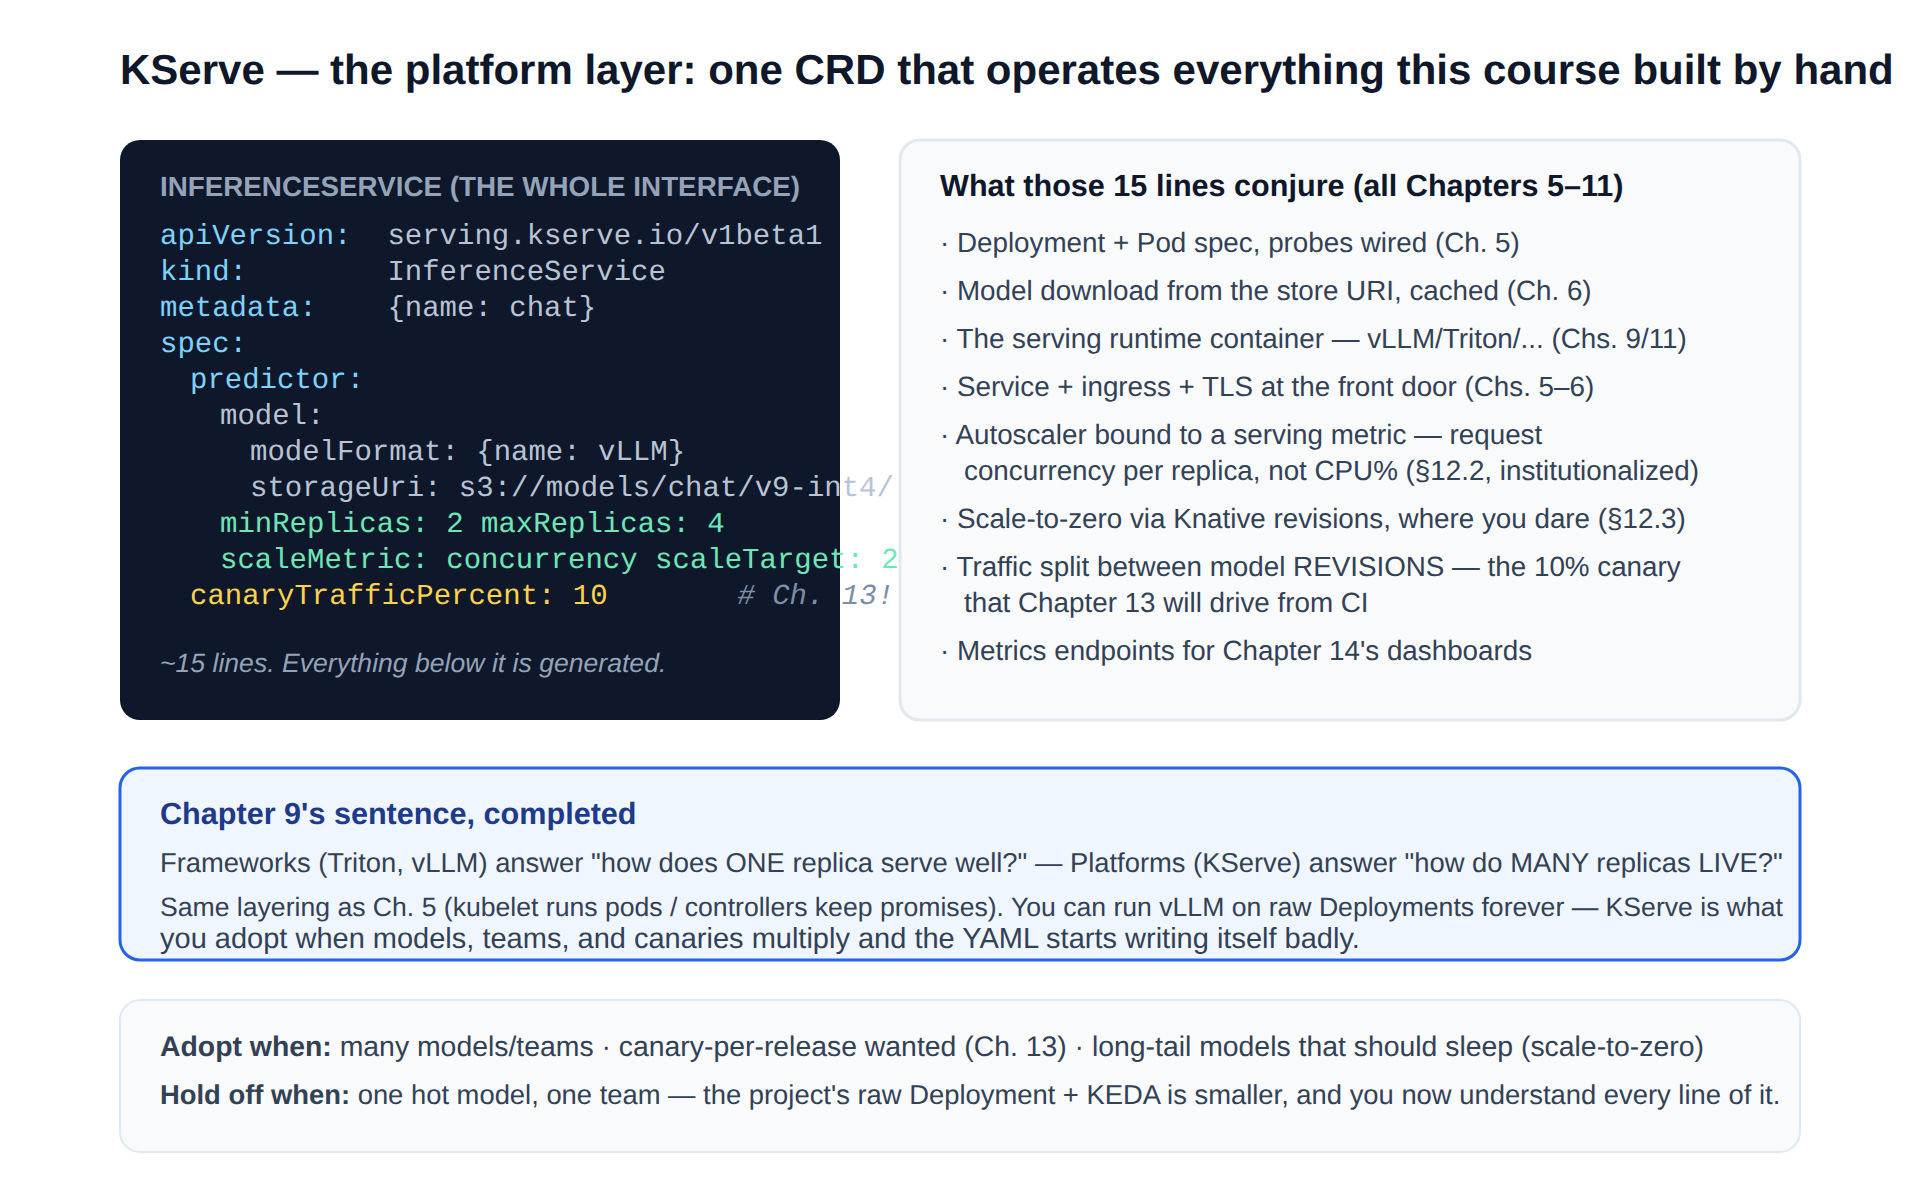
\includegraphics{figures/fig12-5_kserve.png}}\\[3pt]
  \figcaption{Figure 12-5  The CRD and what it conjures. Adopt the platform when models and teams multiply; keep the raw Deployment + KEDA while one hot model is the whole product — you now understand every line it would replace.}
\end{tbbfigure}

The adoption rule mirrors Chapter 9's framework advice, so it will feel familiar: \textbf{adopt the platform when the platform's opinions save you from yaml you were writing badly} — many models, canary-per-release ambitions (Ch. 13), long-tail endpoints that should sleep (§12.3) — and \textbf{hold off while one hot model is the product}, where the project's raw Deployment + KEDA is smaller, fully understood, and one dependency lighter. (Managed endpoints — SageMaker, Vertex — are the same trade with the operator outsourced too; Chapter 13 returns to them.) Either way, notice what KServe institutionalizes: its default scale metric is request \textbf{concurrency per replica}, not CPU — §12.2's argument, promoted from a lesson into a platform default.

\subsection*{The portfolio: buying capacity the way Insull sold it}

Now the money. Everything so far right-sizes \textit{how many} replica-hours you consume; the last lever prices \textit{each hour}, and the menu is Insull's rate card reborn. Clouds sell the same GPU-hour at three prices because they are managing the same problem he was — idle capacity — from the seller's side. \textbf{Committed use} (1–3 year commitments, 30–60\% off) is the base-load tariff: you absorb the idle risk for the floor you know you'll run, and both sides win. \textbf{On-demand} (list price) is the load-following tariff: zero promises, the premium \textit{is} the flexibility. \textbf{Spot/preemptible} (60–90\% off) is the interruptible industrial rate, verbatim: the cloud may shed you at peak with 30 seconds' (GCP) to 2 minutes' (AWS) notice, and the discount is your compensation for engineering around it. The portfolio rule writes itself from Exhibit 12-A's staircase: \textbf{commit the floor, on-demand the shoulder, spot the burst — and never put the floor on spot} (the 03:00 insomniac deserves committed silicon). One more Insull move completes the set: \textbf{off-peak fill}. His night power went to ice houses; your night GPUs go to Chapter 7's batch mode — the re-embedding jobs, the eval sweeps, the calibration runs — work that is interruptible by design and thus spot's truest home, raising load factor without touching the SLO.

\begin{tbbtablewrap}
  \begin{tabular}{@{}>{\raggedright\arraybackslash}m{\dimexpr 0.2181\tbltextwidth-2\tabcolsep\relax} >{\raggedright\arraybackslash}m{\dimexpr 0.1862\tbltextwidth-2\tabcolsep\relax} >{\raggedright\arraybackslash}m{\dimexpr 0.2766\tbltextwidth-2\tabcolsep\relax} >{\raggedright\arraybackslash}m{\dimexpr 0.3191\tbltextwidth-2\tabcolsep\relax}@{}}
  \arrayrulecolor{tbbnavy}\specialrule{1pt}{0pt}{0pt}
  \rowcolor{tbbtablehead}{\centering \bfseries\color{tbbnavy}Tier (grid ancestor)} & {\centering \bfseries\color{tbbnavy}Price vs. list} & {\centering \bfseries\color{tbbnavy}The deal} & {\centering \bfseries\color{tbbnavy}In this course's fleet} \\
  \arrayrulecolor{tbbnavy}\specialrule{0.7pt}{0pt}{2pt}
  {\textbf{Committed (base load)}} & {−30–60\%} & {You own the idle risk for 1–3 yrs} & {The 2-replica floor: 2 × \$595 × 0.60 = \$714/mo} \\
  \arrayrulecolor{tbbtableborder}\hline
  {\textbf{On-demand (load-following)}} & {list} & {Zero promises; premium = flexibility} & {The shoulder the autoscaler adds and removes} \\
  \arrayrulecolor{tbbtableborder}\hline
  {\textbf{Spot (interruptible rate)}} & {−60–90\%} & {30 s–2 min notice; engineer the drain} & {The peak's burst: 13 rep-h/day × \$0.28 ≈ \$113/mo} \\
  \arrayrulecolor{tbbtableborder}\hline
  {\textbf{Off-peak fill (ice houses)}} & {spot, at night} & {Interruptible work in the valley} & {Batch re-embeds, evals, calibration at 03:00} \\
  \arrayrulecolor{tbbnavy}\specialrule{1pt}{2pt}{0pt}
  \end{tabular}\par
  \figcaption{Table 12-2  The rate card, translated. Same GPU-hour, three prices — the difference is who carries the idle risk and who survives an interruption.}
\end{tbbtablewrap}

\subsection*{Serving on spot without tears — the drain drill}

Spot for \textit{serving} (not just batch) is earned, not assumed, and the entire earning is a choreography you already own the pieces of. The interruption notice arrives (a metadata endpoint or node taint); the pod's \textbf{preStop hook + terminationGracePeriodSeconds} (Chapter 5's graceful-shutdown machinery, finally load-bearing) flips readiness to stop new admissions, lets in-flight streams finish — Chapter 11 measured your longest honest stream; that number \textit{is} your grace period — and deregisters from the LB. \textbf{Statelessness pays its final dividend} (Chs. 6/11): a stream that cannot finish re-prefills on another replica — a latency blip, never a wrong answer, the same property that made rollouts and prefix-cache misses safe. Diversify spot pools across zones/instance types (capacity-optimized allocation), and configure the fallback: when spot is reclaimed and not replaced, the autoscaler fills the gap with on-demand — you lose the discount for an hour, not the SLO. Run the drill in staging until an interruption is boring. \textbf{The one absolute rule: spot is a burst tier, never the floor} — the checklist's red flag exists because someone always tries.

\subsection*{The ledger closes — and Chapter 1's break-even with it}

\begin{terminalbox}
\begin{Verbatim}[breaklines=true,breakanywhere=true,fontsize=\small,formatcom=\color{tbbtermfg},codes=\tbbcodeactive]
$ python fleet_ledger.py --final          # the course's bill, walked
 Wk 7  estimated, 8 x L4, 24/7             $4,762   # the syllabus bill
 Wk 10 INT8: 2x goodput -> 4 replicas      $2,381   # same SLO
 Wk 12 autoscale: 61 rep-h/day             $1,513   # same SLO
 Wk 12 portfolio:
   commit floor  2 x $595.20 x 0.60      $  714.24
   spot burst    403 rep-h x $0.28       $  112.84
   pre-warm + cron cushion               $   49.60
   TOTAL                                 $  876.68   < $900 ceiling

 unit economics (measured, Wk 11 sweeps):
   capacity  ~3.1B tok/mo   served ~2.0B tok/mo  (load factor again!)
   $/M tokens: 876.68 / 2000 = $0.44   vs API $0.50: self-host wins
   ...at THIS utilization. at half the traffic, the API wins. Ch. 1's
   break-even curve: closed, with measured numbers, 11 weeks later.
\end{Verbatim}
\end{terminalbox}
\figcaption{Transcript 12-6  The finish line. \$4,762 → \$2,381 (optimization) → \$1,513 (autoscaling) → \$877 (portfolio) — under the Week 1 ceiling with \$23 to spare, every step a measured lever. And the \$/M-token line closes the build-vs-buy question the course opened with: the answer was never a slogan, it was a utilization.}

Three habits turn that one-time victory into \textbf{FinOps} — the ongoing discipline rather than the heroic afternoon. \textbf{Meter the unit, not the total}: the bill that matters is \$/M tokens (or \$/K requests), because it is comparable across weeks, models, and against the API alternative; total spend only tells you the product grew. \textbf{Tag and show back}: every resource carries team/model/env labels so the ledger decomposes — Chapter 6's NAT-trap story (\$5k/yr, silent) is the canonical example of spend that hides in untagged plumbing. \textbf{Alarm the anomaly}: a budget alert at 80\%/100\%/120\% of forecast (the Ch. 2 lab guardrail, graduated to production) catches the leaked GPU, the forgotten dev fleet, the retry storm billing as traffic. None of this is glamorous; all of it is the difference between the \$877 staying \$877 and the ghost GPUs quietly returning. Insull's real product, a century on, is still the same: \textbf{watched capacity.}

\begin{calloutbox}{tbbred}{tbbxFEF2F2}
{\normalsize\bfseries\color{tbbx991B1B}Box 12-1  Cost-review red flags — the checklist, published}\par\vspace{3pt}
\begin{tbbitemize}
  \item \textbf{No unit cost} — total spend without \$/M tokens is a growth chart, not a cost review.
  \item \textbf{Commitments sized to the peak} — you just bought the idle back; commit the FLOOR, portfolio the rest.
  \item \textbf{Spot under the floor} — the discount that pages you at 03:00; burst tier only, drain drill rehearsed.
  \item \textbf{A flat replica line in the traffic graph} — Exhibit 12-A is a one-glance diagnosis; load factor belongs on the dashboard.
  \item \textbf{Untagged spend / silent plumbing} — the NAT trap, the forgotten dev fleet, the zombie volume: if it can't be attributed, it can't be reviewed.
  \item \textbf{Savings claimed without an SLO citation} — every dollar cut must name the clause it didn't break (this chapter halved the bill at the SAME SLO; that sentence is the whole discipline).
\end{tbbitemize}
\end{calloutbox}

\vspace{3.0pt}

\begin{calloutbox}{tbbpurple}{tbbpurplefill}
{\normalsize\bfseries\color{tbbpurple}Think About It}\par\vspace{3pt}
\begin{tbbitemize}
  \item Rebuild Transcript 12-6 under a traffic doubling (peak 208 streams, same shape): staircase, rep-h/day, portfolio split, final bill, and \$/M tokens. Which line improves, which worsens, and why does the unit cost FALL as the product grows (Insull would know)?
  \item Your commitment covers 2 replicas for 1 year, and month 4 brings the INT4 build (§11.5): each replica now serves 1.6× the streams. Are you over-committed? Walk the options (grow into it, shift floor workloads, resell/modify) — and derive the planning rule for committing under an optimization roadmap.
  \item The KServe canary field splits traffic 90/10 — but §10.3's gate already decided the INT4 model was safe. What does the canary check that the gate cannot? (Think: real traffic distribution, real infrastructure, real SLOs.) This is Chapter 13's opening argument — draft it in three sentences.
  \item Compute the break-even API price for YOUR project from the lab's ledger: at what \$/M tokens does self-hosting stop winning, and which single input (utilization, GPU price, tokens/replica) moves that answer most? Present it as the one-slide answer to "why don't we just use the API?"
\end{tbbitemize}
\end{calloutbox}

\section{Lab: The Project Midpoint — Make It Breathe, Then Present the Ledger}

The syllabus names this week's deliverable plainly: \textbf{팀 프로젝트 중간 점검} — the team project's midpoint review. The lab therefore has two parts. Part A (hands-on, \textasciitilde{}90 minutes) makes a fleet breathe in front of you and prices its reflexes; Part B assembles everything since Week 7 into the eight-minute package your team presents — the same package, not incidentally, that a staff engineer would bring to a capacity review. Budget: \textasciitilde{}\$3 of GPU time, plus the billing screenshot whose ritual this chapter finally explains from the inside.

\begin{tbbfigure}
  \adjustbox{max width=0.94\linewidth,max totalheight=0.46\textheight}{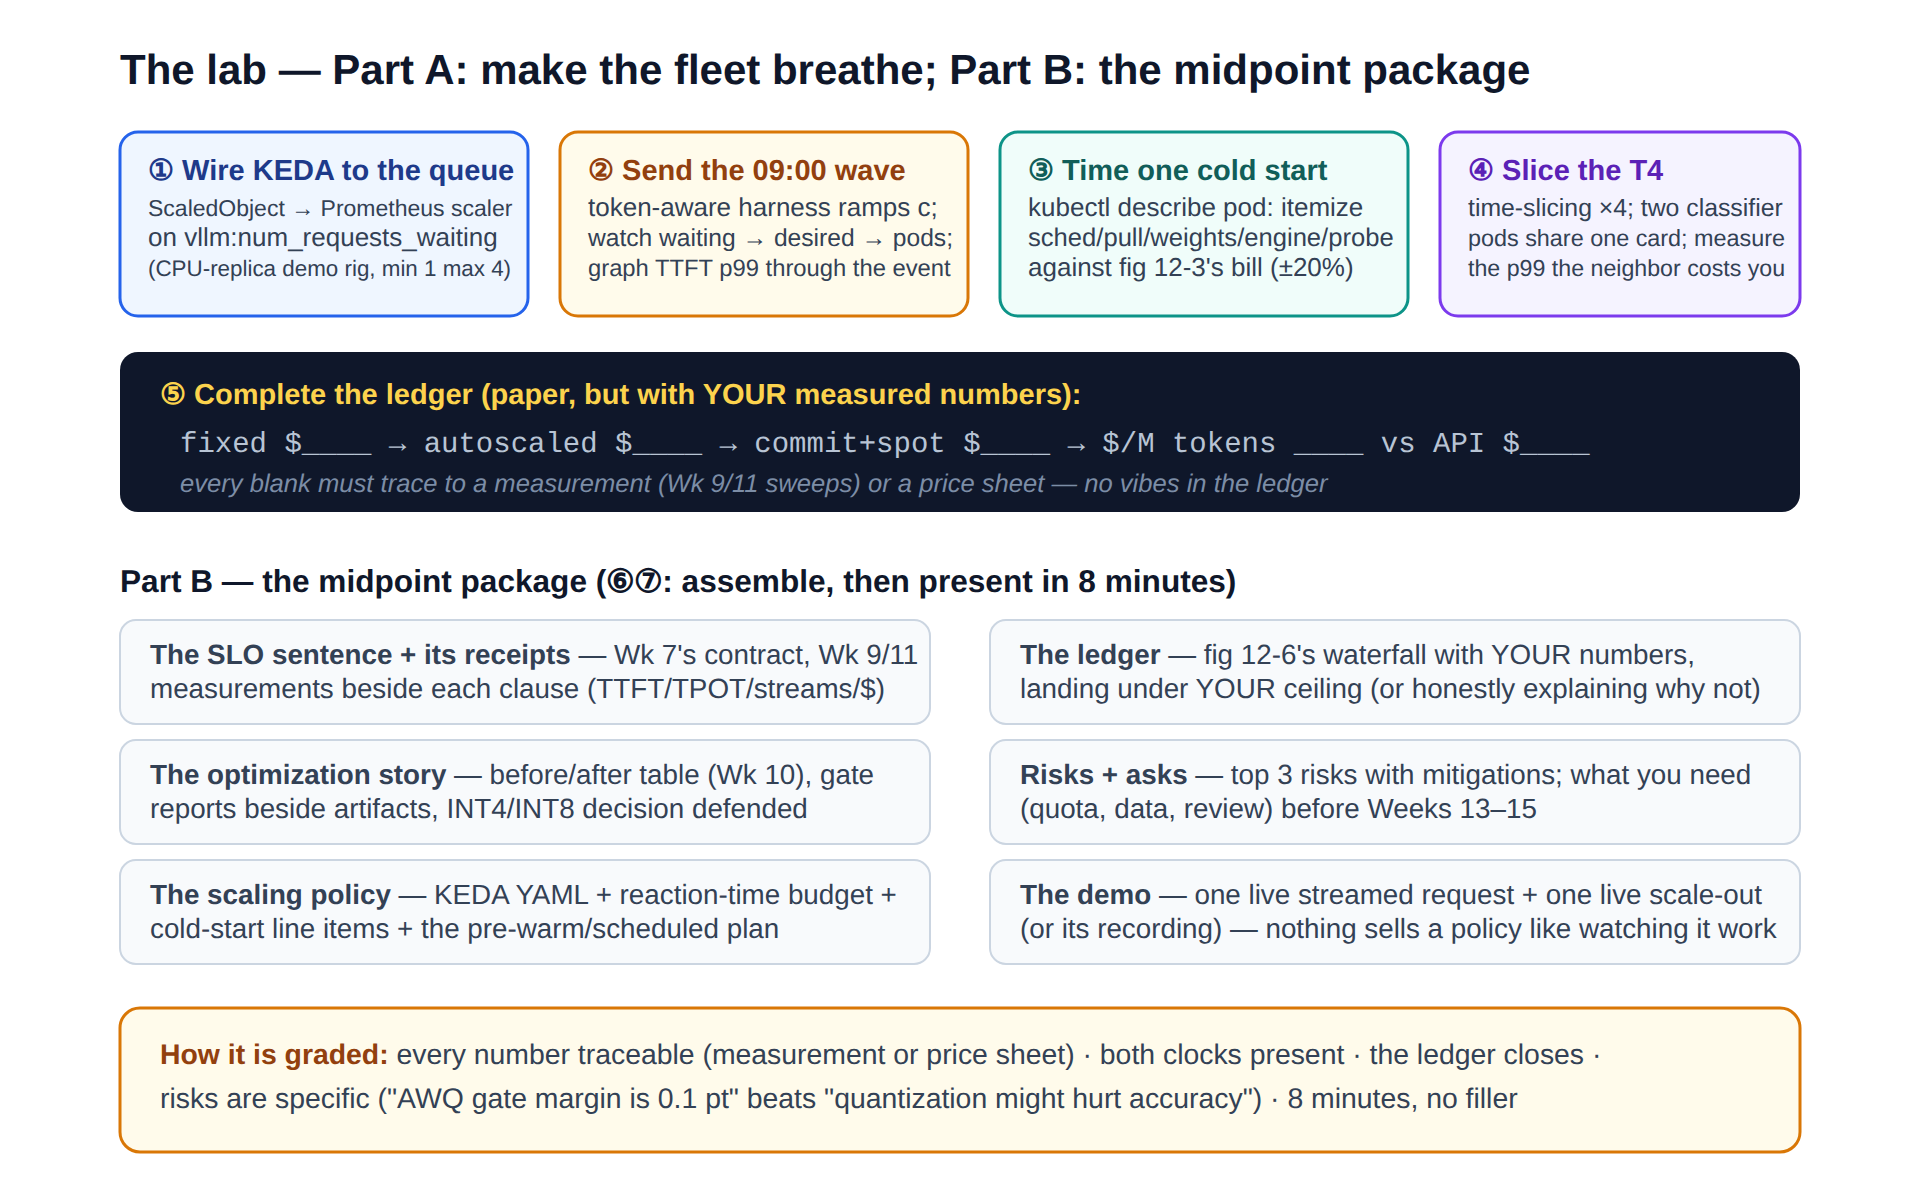
\includegraphics{figures/fig12-7_midpoint.png}}\\[3pt]
  \figcaption{Figure 12-7  The lab's two parts. A: wire the scaler, send the wave, time a birth, slice the T4 — four measurements. B: the midpoint package — six artifacts, every number traceable, eight minutes.}
\end{tbbfigure}

\subsection*{Part A — four measurements (①–⑤)}

\begin{tbbitemize}
  \item \textbf{① Wire KEDA to the queue.} Deploy the handout's demo rig (CPU-mode replicas so scaling is visible without four GPUs): Prometheus + KEDA + Transcript 12-1's ScaledObject on \code{vllm:num\_requests\_waiting}, min 1 / max 4. Confirm the HPA object KEDA generates — you are managing a manager (Ch. 5's pattern, one level up).
  \item \textbf{② Send the 09:00 wave.} Chapter 11's token-aware harness ramps concurrency; watch \code{waiting → desired → pods} with three terminals (\code{kubectl get hpa -w}, \code{get pods -w}, the harness's TTFT log). Graph TTFT p99 through the event; annotate detection, birth, drain. Then add the 08:40 cron trigger and send the identical wave — two graphs, one lesson, \textasciitilde{}\$0 of GPU.
  \item \textbf{③ Time one real birth.} On the GPU node, delete the vLLM pod and stopwatch Transcript 12-3's line items from \code{kubectl describe pod} + engine logs. Reconcile each line with its owning chapter (±20\%); name your fleet's dominant line and the ladder rung that attacks it. This number goes in the midpoint package as \textit{your} reaction-time budget.
  \item \textbf{④ Slice the T4 and measure the rent.} Apply the time-slicing ConfigMap (replicas: 4), co-schedule two classifier pods, re-run the Week 9 sweep alone-vs-neighbored (Transcript 12-4). Report p50, p99, and req/s@SLO for both — and write the one-sentence verdict on time-slicing under an SLO.
  \item \textbf{⑤ Close the ledger.} Fill Transcript 12-6's blanks with \textit{your} measured numbers: your staircase (from any real day of metrics, or the handout's replay), your rep-h/day, your portfolio split from live price sheets, your \$/M tokens against the API alternative. Every blank must trace to a measurement or a price sheet — the graders' first check.
\end{tbbitemize}

\subsection*{Part B — the midpoint package (⑥–⑦)}

Assemble six artifacts, then rehearse to eight minutes. \textbf{The SLO sentence with receipts} — Week 7's contract, rewritten in Week 11's clauses, with the measurement that certifies each clause beside it. \textbf{The optimization story} — Week 10's before/after table, gate reports beside artifacts, the INT4/INT8 decision defended in one paragraph. \textbf{The scaling policy} — your ScaledObject, your reaction-time budget from ③, the cron/pre-warm plan, and the one graph from ② that shows the wave survived. \textbf{The ledger} — Figure 12-6's waterfall with your numbers, landing under your ceiling, or honestly explaining the gap and the plan. \textbf{Risks and asks} — three specific risks with mitigations ("AWQ gate margin is 0.1 pt on the safety slice" beats "quantization might hurt accuracy"), and what you need before Weeks 13–15. \textbf{The demo} — one live streamed request and one live scale-out (or its recording). Present; collect the feedback; it is Week 15's dress rehearsal.

\begin{calloutbox}{tbbteal}{tbbxF0FDFA}
{\normalsize\bfseries\color{tbbx115E59}Box 12-2  The midpoint rubric — how the eight minutes are graded}\par\vspace{3pt}
\begin{tbbitemize}
  \item \textbf{Traceability (40\%)} — every number cites a sweep, a transcript, or a price sheet. "About 500" with no source is the only failing answer in this course.
  \item \textbf{Both clocks present (20\%)} — TTFT and TPOT with percentiles and load stated; a single "latency" forfeits the row (Box 11-2 lives on).
  \item \textbf{The ledger closes (20\%)} — fixed → autoscaled → portfolio → unit cost, arithmetic checkable in real time; under-ceiling earns nothing extra, \textit{un-explained} gaps cost.
  \item \textbf{Risks are engineering (10\%)} — specific, measured, mitigated; and at least one must be a cost risk (commitment vs. roadmap, spot availability, egress).
  \item \textbf{Time discipline (10\%)} — eight minutes, then questions. Staff engineers who cannot stop talking get their capacity reviews rescheduled; so will you.
\end{tbbitemize}
\end{calloutbox}

\vspace{3.0pt}

Deliverables: the four Part-A measurement artifacts (two wave graphs, the itemized birth, the neighbor-tax table), the completed ledger, the six-artifact package as slides or a doc, and — for the last technical time in this course — the billing screenshot, which after this chapter is no longer a ritual but a \textbf{statement you can read}: every line item on it now has a chapter, a lever, and an owner. That was the point all along.

\begin{calloutbox}{tbbpurple}{tbbpurplefill}
{\normalsize\bfseries\color{tbbpurple}Think About It}\par\vspace{3pt}
\begin{tbbitemize}
  \item Your ② graphs show the cron run's TTFT p99 flat at 0.46 s but cost +\$1.07/day, while the reactive run breached for 3 min at \$0 extra. Write the two-sentence recommendation for YOUR product — and name the product fact (not the infra fact) that decides it.
  \item In ③ your birth came to 190 s, not 150: the extra 40 s is image pull (no node cache — first pod on a fresh node). Which ladder rungs fix it, what does each cost monthly, and which do you actually recommend given your fleet churns nodes twice a week?
  \item The midpoint reviewer asks: "Your ledger assumes the diurnal shape holds. What breaks if a B2B customer adds a nightly batch of 50k requests at 02:00?" Answer with the staircase, the portfolio (which tier serves it?), and the load-factor consequence — then explain why this is GOOD news for your unit cost.
  \item Write your team's three risk lines now, as a draft: one SLO risk (from Wk 9/11 measurements), one cost risk (from this chapter's ledger), one delivery risk (Weeks 13–15). Apply the rubric's specificity bar to your own sentences and revise once.
\end{tbbitemize}
\end{calloutbox}

\namedsection{Summary}{The Chapter in Sixteen Points}

\qitem{1}{\textbf{The waste is structural, not a misconfiguration.} Demand has a shape in time; a static fleet is a horizontal line. Exhibit 12-A, measured: needed 61 replica-hours/day, paid 96 — load factor 63.5\%, \$868/month of night shift. Exhibit 1-B's ghost GPU, diurnal edition.}

\qitem{2}{\textbf{This is 1902's problem, solved by 1910.} Samuel Insull ran Chicago's grid on load factor (average ÷ peak): meter demand, interlock customers' peaks, sell the valley cheap, shed interruptibles at peak. Every mechanism this chapter taught is one of his moves — autoscaling, sharing, spot, night batch.}

\qitem{3}{\textbf{An autoscaler is a thermostat, not a meteorologist:} every 15 s, desired = ceil(current × metric ÷ target), written into one integer that Chapter 5's machinery obeys. The engineering is the metric and the stopwatch, not the formula.}

\qitem{4}{\textbf{Scale on demand signals, not supply gauges.} CPU\% never fires for a GPU service (9\% while the GPU drowns — Ch. 9's exhibit, mirrored); GPU util\% saturates and lies at partial load. The right eye is the admission queue (vllm:num\_requests\_waiting): leading, unbounded, and what users feel (L = λW).}

\qitem{5}{\textbf{Temper the loop asymmetrically:} scale up on the instant signal, scale down only on a trailing window (stabilization/cooldown \textasciitilde{}300 s). The loss function is asymmetric — eager-up wastes replica-minutes, eager-down breaks the SLO. Flapping converts your bill into cold-start overhead (Ch. 10's torch.compile spiral).}

\qitem{6}{\textbf{Reaction time is part of capacity:} T = detect (≤15 s) + decide (≤15 s) + birth (\textasciitilde{}150 s warm-node). The queue integrates the excess for all of T — the 09:00 wave breaches TTFT for three minutes on the reactive path, or is deleted by an 08:40 cron for \$1.07. Calendar beats clairvoyance for peaks you can see.}

\qitem{7}{\textbf{Pods chase waves; nodes follow forecasts.} A GPU node birth is 3–7 min and sometimes "no capacity" — never on the SLO path. Pre-provision the day's node envelope; autoscale pods inside it.}

\qitem{8}{\textbf{The cold start is a bill, itemized:} schedule 2 s + image 16 s (Ch. 4) + weights 9 s (Ch. 6) + engine init 95 s (Ch. 11) + warm-up 28 s (Chs. 5/10) = 150 s. Firecracker's 125 ms solved the ENVIRONMENT line; the payload lines are yours. Serverless GPU = warm pools + snapshot/restore of initialized processes, at a premium.}

\qitem{9}{\textbf{The mitigation ladder is chapters you own:} slim/cached/lazy images → parallel weight fetch + node cache → warm-up inside readiness → +1 headroom (\textasciitilde{}\$50/mo) → scheduled scaling → scale-to-zero. Zero is for endpoints whose callers absorb minutes of first-hit latency: the long tail sleeps, the SLO-bearing head keeps a floor of 2 (rollouts + the 03:00 user).}

\qitem{10}{\textbf{Sharing bends the one-tenant-per-card rule three ways:} time-slicing (turns on the whole die — no isolation; dev only; the lab measured p99 9.8 → 38.4 ms with one neighbor), MPS (concurrent, one blast radius — your own small models), MIG (hardware partitions, up to 7 per big die — own SMs/L2/DRAM/OOM: SLO-safe multi-tenancy; not on T4/L4).}

\qitem{11}{\textbf{The consolidation math is Insull's diversity trick:} a 1g.10gb A100 slice (≈\$0.51/hr) matches a whole T4 (\$0.53) with six slices left — IF the tenants' peaks interlock and the slice passes its own §10.2 diagnosis (1/7 the bandwidth). Correlated peaks re-create the 13:00 problem one level down.}

\qitem{12}{\textbf{KServe is the platform species Chapter 9 named:} one 15-line InferenceService conjures Deployment, probes, model fetch, runtime, ingress, a concurrency-based autoscaler, scale-to-zero, and a canary traffic split. Adopt when models/teams multiply; hold the raw Deployment + KEDA while one hot model is the product.}

\qitem{13}{\textbf{Buy capacity as a portfolio:} commit the floor (−30–60\%), on-demand the shoulder, spot the burst (−60–90\%, 30 s–2 min notice), fill the valley with batch. Never the floor on spot. The drain drill is Chapter 5's preStop + Chapter 11's statelessness: finish streams, deregister, re-prefill elsewhere — a blip, never a wrong answer.}

\qitem{14}{\textbf{The ledger closed under the ceiling:} \$4,762 (Wk 7, estimated) → \$2,381 (Wk 10, INT8) → \$1,513 (autoscale, 61 rep-h/day) → \textbf{\$877} (= \$714 committed + \$113 spot + \$50 pre-warm) < \$900 — every step a measured lever at the SAME SLO.}

\qitem{15}{\textbf{Unit economics close Chapter 1's break-even:} \$877 ÷ 2.0B served tokens = \$0.44/M vs. the API's \$0.50 — self-hosting wins at THIS utilization and loses at half of it. Build-vs-buy was never a slogan; it was a load factor.}

\qitem{16}{\textbf{FinOps is watched capacity:} meter \$/M tokens (not totals), tag and show back (the NAT trap hides in untagged plumbing), alarm the anomaly (80/100/120\% of forecast). The midpoint package presents all of it in eight minutes, every number traceable — Week 15's dress rehearsal.}

\namedsection{Exercises}{}

\subsection*{A. Multiple choice}

\qitem{1}{A GPU chat service is drowning (queue growing, TTFT red) but its CPU-based HPA never scales. The root cause is:}

\begin{tbboptions}
  \item ① The HPA loop is too slow        ② The contended resource (GPU/queue) is invisible to the metric being watched — CPU idles at 9\%
  \item ③ maxReplicas is too low        ④ The image is too large
\end{tbboptions}

\qitem{2}{The best autoscaling metric for a vLLM fleet is num\_requests\_waiting because it is:}

\begin{tbboptions}
  \item ① Cheapest to collect        ② Leading (fires before latency moves), unbounded (says how wrong capacity is), and user-felt (the queue is TTFT's numerator)
  \item ③ Built into Kubernetes        ④ Always zero at steady state
\end{tbboptions}

\qitem{3}{Scale-up windows are instant while scale-down windows are \textasciitilde{}5 minutes because:}

\begin{tbboptions}
  \item ① Scaling down is mechanically slower        ② The loss function is asymmetric: eager-up wastes replica-minutes; eager-down breaks the SLO and re-pays cold starts (flapping)
  \item ③ Kubernetes requires it        ④ Billing is per 5 minutes
\end{tbboptions}

\qitem{4}{With 2 replicas, 41 total waiting, and a target of 10 per replica, the HPA computes desired =}

\begin{tbboptions}
  \item ① 3        ② 4        ③ ceil(2 × 20.5 ÷ 10) = 5 (then capped by maxReplicas)        ④ 41 ÷ 10 = 4.1 → 4
\end{tbboptions}

\qitem{5}{Firecracker's 125 ms microVM did NOT solve the GPU cold start because:}

\begin{tbboptions}
  \item ① It only runs on CPUs        ② The bill is payload, not environment: gigabytes of image and weights, CUDA context, engine init — 148 of the 150 seconds
  \item ③ Kubernetes cannot use microVMs        ④ GPUs boot slowly
\end{tbboptions}

\qitem{6}{Scale-to-zero is appropriate for:}

\begin{tbboptions}
  \item ① Any service with idle hours        ② The chat fleet at night
  \item ③ Endpoints whose callers can absorb minutes of first-hit latency — the long-tail internal model, the dev endpoint, the batch-triggered scorer        ④ Nothing on GPUs
\end{tbboptions}

\qitem{7}{A team puts two SLO-bearing services on one time-sliced GPU. The predictable outcome is:}

\begin{tbboptions}
  \item ① 2× throughput        ② Nothing changes
  \item ③ p50 roughly holds while p99 multiplies (the unlucky request eats the neighbor's slice) — and one tenant's OOM kills both        ④ MIG activates automatically
\end{tbboptions}

\qitem{8}{The portfolio rule for the diurnal staircase is:}

\begin{tbboptions}
  \item ① Everything on spot for the discount        ② Everything committed for the discount
  \item ③ Commit the floor, on-demand the shoulder, spot the burst — and never the floor on spot        ④ On-demand only; pricing games are not engineering
\end{tbboptions}

\subsection*{B. Short answer}

\qitem{1}{Define load factor for a GPU fleet, compute it for Exhibit 12-A (61 needed, 96 paid), and name the 1900s figure who ran a utility on the metric.}

\qitem{2}{Write the desired-replica formula and evaluate it for: 3 replicas, 66 waiting total, target 15 per replica, maxReplicas 6.}

\qitem{3}{Itemize the 150-second warm-node cold start (five line items with owning chapters), and name the line that dominates a vLLM fleet.}

\qitem{4}{Time-slicing vs. MPS vs. MIG in one sentence each, keyed to what each isolates (or doesn't).}

\qitem{5}{State the spot drain drill's four beats and the Chapter 11 property that makes an interrupted stream a blip rather than a wrong answer.}

\qitem{6}{Why does the midpoint ledger report \$/M tokens instead of monthly spend? Give both reasons (comparability + the Ch. 1 question it answers).}

\subsection*{C. Essay}

\qitem{1}{The capacity-review essay: your service peaks at 340 concurrent streams (11:00–15:00 weekdays), shoulders at 120, floors at 25 overnight and weekends. Per-replica: 32 seats, \$1.10/hr, cold start 3 min. Build the staircase, the reaction plan (cron + queue triggers + headroom), the portfolio (commit/on-demand/spot with a 1-yr commit at −38\%, spot at −64\%), and the final monthly bill — then state the load factor before and after, Insull-style.}

\qitem{2}{Defend or attack: "Autoscaling is the least interesting lever in this chapter — the real money was in Chapters 10 and 11, and the real risk is here." Use the course ledger (\$4,762 → \$2,381 → \$1,513 → \$877), the SLO-breach modes each lever introduces, and the engineering cost of each step. Where does the marginal dollar of engineering effort go next for THIS project?}

\qitem{3}{The consolidation essay: a department runs nine small models, each on its own T4 (\textasciitilde{}\$0.53/hr, duty cycles 5–40\%, three teams, two SLO-bearing). Design the target fleet across time-slicing/MPS/MIG/whole cards: placement per model class, the isolation argument for each choice, the blast-radius and reconfiguration-drain risks, and the monthly before/after. Name the one measurement you would demand before signing off (hint: Insull's requirement).}

\qitem{4}{The break-even essay: using the final ledger (\$877, 2.0B served tokens, capacity 3.1B), derive the self-host vs. API decision as a function of monthly tokens. Compute the crossover against a \$0.50/M API, show how INT4 (1.6×) and a traffic doubling each move it, and close with a one-paragraph memo for a startup at 0.4B tokens/month.}

\namedsection{Answers and Commentary}{}

\subsection*{A. Multiple choice}

\qitem{1}{\textbf{②} The autoscaler's eye watches a resource that isn't contended. Ch. 9's Exhibit A mirrored: there CPU pinned while the GPU idled; here the GPU drowns while CPU naps. Scale on demand signals. (§12.2)}

\qitem{2}{\textbf{②} All three properties in one metric — and it is the same line Chapter 11 taught you to read and Transcript 11-3 watched. Supply gauges (CPU\%, GPU\%) fail at least one of the three. (§12.2)}

\qitem{3}{\textbf{②} The asymmetry encodes the loss function: replica-minutes vs. SLO breach + re-paid births. Flapping's worst case is Ch. 10's think-box (compile-on-scale-out). (§12.2)}

\qitem{4}{\textbf{③} Per-replica metric is 20.5; desired = ceil(2 × 20.5/10) = ceil(4.1) = 5; the cap then applies. ④ is the classic error — the formula scales the CURRENT count, it doesn't divide the raw total. (§12.2)}

\qitem{5}{\textbf{②} Transcript 12-3: the environment contributes \textasciitilde{}2 s of 150. Firecracker solved 2005's problem brilliantly; 2026's problem is gigabytes and CUDA context — warm pools and snapshots, not faster boots. (§12.3)}

\qitem{6}{\textbf{③} The decision rule is the caller's latency tolerance, not the idle hours. (a) fails it — the 03:00 user is real and the floor also serves rollouts. (§12.3)}

\qitem{7}{\textbf{③} Transcript 12-4, measured: p50 3.1 ms, p99 38.4 ms — the tail eats the context switches and the neighbor's batches; VRAM is communal. Time-slicing under an SLO is a Ch. 14 war story on layaway. (§12.4)}

\qitem{8}{\textbf{③} The staircase maps to the rate card tier by tier; the floor on spot is the checklist's reddest flag (a 03:00 reclamation with no replacement capacity). (§12.5)}

\subsection*{B. Short answer}

\qitem{1}{Load factor = needed (or average) ÷ paid (or peak) capacity-hours: 61/96 = \textbf{63.5\%}. Samuel Insull, Chicago Edison — who priced power on demand curves and filled valleys to raise exactly this number. (§12.1)}

\qitem{2}{desired = ceil(current × metric ÷ target) = ceil(3 × 22 ÷ 15) = ceil(4.4) = \textbf{5} (≤ max 6, so 5 stands). Per-replica metric = 66/3 = 22. (§12.2)}

\qitem{3}{Schedule 2 s (Ch. 5) + image pull 16 s (Ch. 4) + weights 9 s (Ch. 6) + \textbf{engine init 95 s (Ch. 11 — VRAM load, KV pool, CUDA graphs; the dominant line)} + probe warm-up 28 s (Chs. 5/10) = 150 s. (§12.3)}

\qitem{4}{Time-slicing: tenants take turns on the whole die — isolates nothing. MPS: tenants run concurrently with SM caps — isolates compute shares, not bandwidth or faults. MIG: hardware partitions with own SMs/L2/DRAM/OOM — isolates nearly everything, at 1/7 granularity on big dies only. (§12.4)}

\qitem{5}{Notice → stop admitting (readiness off) → finish in-flight streams within the grace period → deregister. Statelessness (full history in each request; KV is a cache, not a contract): the reclaimed stream re-prefills elsewhere — latency blip, correct answer. (§12.5, Chs. 5/11)}

\qitem{6}{Unit cost is comparable — across weeks, models, fleet sizes, and against the API's posted \$/M — while total spend only measures growth. And it is the direct answer to Chapter 1's build-vs-buy: \$0.44 vs. \$0.50 at this utilization. (§12.5)}

\subsection*{C. Essay (grading points)}

\qitem{1}{Staircase: peak ceil(340/32)=11 (4 h), shoulder ceil(120/32)=4 (\textasciitilde{}8 h weekdays), floor ceil(25/32)=1→\textbf{2} (ops floor) → \textasciitilde{}76 rep-h/weekday, \textasciitilde{}48 weekend. Reaction: cron to 11 at 10:40 (3-min births!), queue trigger for shape, +1 headroom 11:00–15:00. Portfolio: commit 2 (−38\%), on-demand shoulder, spot the 7-replica burst (−64\%). Strong answers show the arithmetic landing near: fixed 11×24 = 264 rep-h/day vs. \textasciitilde{}72 average → LF \textasciitilde{}27\% → \textasciitilde{}64\% after. Credit any consistent bill; penalize floors on spot or node births inside the wave. (§§12.1–12.5)}

\qitem{2}{Strong essays split "interesting" from "valuable": autoscaling's \$868/mo (2,381→1,513 is the scaler; 1,513→877 is portfolio) vs. Ch. 10's \$2,381 — optimization won more; but autoscaling's risk profile is unique (it can CAUSE breaches: flapping, cold-start ambush, wrong metric), so its engineering is mostly safety. The marginal dollar: for this project, likely §12.3's engine-init line (95 s) or the ledger's served/capacity gap (marketing, not infra!). Reward essays that notice the levers compose multiplicatively and that the SLO-breach citation discipline (Box 12-1) is the actual thesis. (chapter-wide)}

\qitem{3}{Look for: SLO-bearing pair → MIG slices (or whole cards if peaks correlate); one-team clusters of tiny models → MPS; dev/notebooks → time-slicing; anything filling its card → whole card. Risks: node-level blast radius (anti-affinity across the two SLO models), MIG reshape drains (profile per node pool), slice bandwidth vs. each model's §10.2 diagnosis. The demanded measurement: \textbf{peak-correlation across the nine duty cycles} (Insull's diversity) — consolidation on correlated peaks re-creates the problem. Before/after ≈ 9 × \$394 → 1 A100 (\textasciitilde{}\$2,678) + 1–2 whole cards, if and only if diversity holds. (§12.4)}

\qitem{4}{Self-host ≈ fixed floor + variable rep-h: near-linear in tokens ABOVE the floor, flat below it — so unit cost falls with volume (Insull). Crossover vs. \$0.50/M with the course numbers lands near \textasciitilde{}1.7–1.8B tokens/mo (floor-dominated below, portfolio-priced above); INT4 shifts it down \textasciitilde{}1.6× (more tokens per rep-h), doubling traffic rides the same fleet to \$0.28/M. At 0.4B/mo: the API wins \textasciitilde{}2× — memo should say "buy now, revisit at \textasciitilde{}1.5B/mo or when data-governance forces self-host," and cite the two inputs that dominate (utilization, tokens/replica). Any consistent arithmetic earns full credit; slogans earn none. (§12.5, Ch. 1 §1.5)}

\namedsection{Further Reading}{}

Entries tagged \textbf{[This week]} support the lab directly; \textbf{[Wk N]} marks material that pays off later.

\begin{tbbitemize}
  \item \textbf{[This week] Kubernetes HPA documentation — "Horizontal Pod Autoscaling" (algorithm + behavior/stabilization)} and \textbf{KEDA docs — ScaledObject, Prometheus scaler, cron scaler} — Transcripts 12-1/12-2's authoritative sources; the behavior stanza is §12.2's temper, verbatim.
  \item \textbf{[This week] NVIDIA MIG User Guide · GPU Operator time-slicing docs} — Chapter 2 §2.6 promised these would become hands-on this week: profiles, K8s device-plugin strategies, and the reconfiguration-drain caveat, operationally.
  \item \textbf{[This week] KServe documentation — InferenceService \& autoscaling} — Chapter 9's "skim the CRD, deploy it in Week 12," now due; the concurrency-based default is §12.2 institutionalized.
  \item \textbf{A. Agache et al., "Firecracker" (NSDI 2020), re-read §§1–2} — Week 2's required reading, second pass: this time read it asking "which of MY 150 seconds does this solve?" The answer being "two of them" is the §12.3 lesson.
  \item \textbf{Cloud provider docs: Spot best practices (AWS) / Preemptible \& Spot VMs (GCP) · committed-use discounts / Savings Plans} — the portfolio's fine print: notice windows, capacity-optimized allocation, commitment scopes. Read before signing anything §12.5-shaped.
  \item \textbf{J. F. Wasik, "The Merchant of Power" (2006)} — the Insull biography: load factor, demand meters, interlocking peaks, and the invention of utility economics — this chapter's anchor story at book length (and a cautionary ending the chapter omitted).
  \item \textbf{"Sub-second GPU cold start"-class engineering posts (Modal, Fly.io, Cloud Run GPU) + containerd lazy-pull (eStargz) docs} — Chapter 4 promised these as the cold-start frontier: snapshot/restore, image streaming, warm-pool economics.
  \item \textbf{[This week, fun] Your cloud console's billing page, sorted descending} — find the NAT gateway (Ch. 6), the idle dev GPU, the untagged mystery. After this chapter it reads as a statement, not a ritual: every line has a lever and an owner.
\end{tbbitemize}

\vspace{5.0pt}

\begin{calloutbox}{tbbblue}{tbbbluefill}
{\normalsize\bfseries\color{tbbblue}Next chapter — Chapter 13: MLOps and Deployment Automation}\par\vspace{3pt}
The fleet now breathes and the bill now closes — but every improvement this course has shipped was deployed by \textbf{a human typing kubectl}, and Transcript 12-5 left a knob dangling: \code{canaryTrafficPercent: 10}, a traffic split with nobody driving it. Chapter 13 builds the driver: \textbf{model registries and versioning} (Ch. 4's digests and Ch. 6's store, grown into a promotion workflow), \textbf{CI/CD pipelines} that run Chapter 10's gates and Chapter 9's sweeps on every candidate (GitHub Actions, in the lab), \textbf{canary, A/B, and shadow deployment} — what the 10\% split checks that the offline gate cannot — and a clear-eyed look at \textbf{managed endpoints} (SageMaker, Vertex AI): the same platform trade as KServe with the operator outsourced too. The goal is the one sentence every on-call engineer wants true: \textit{the deploy is boring.}
\end{calloutbox}
